% =====================================================================
% paper11_forecasting_baselines_v68.tex
% Forecasting against naive benchmarks: a scored test of process-based
% modules on Northern cod and the Edwards Aquifer
% Author: Amin Abaee (Independent Researcher, Tehran, Iran)
%
% Lineage: v67 is preserved unchanged. This v68 working edition separates the
% Edwards H1/H2 point-score gates from the M2m and Pass-2 function-class
% dispositions, corrects the clipped-path record, and replaces the archived
% cod operating-characteristic estimates with a deterministic, fail-loudly
% rerun. Historical rolling scores and all v67 sources remain preserved.
% Target: Environmental Modelling & Software (elsarticle, author-year).
% Build route and checks are recorded in the v68 README.
% Compiles with pdfLaTeX / XeLaTeX / LuaLaTeX / tectonic.
% =====================================================================
\documentclass[preprint,11pt,authoryear]{elsarticle}

\usepackage{amsmath,amssymb,amsthm}
\usepackage{booktabs}
\usepackage{array}
\usepackage{tabularx}
\usepackage{multirow}
\usepackage{graphicx}
\graphicspath{{./}{figs/}{paper11_forecasting_baselines_v68_src/figs/}}
\usepackage{enumitem}
\usepackage{placeins}
\renewcommand{\topfraction}{0.9}
\renewcommand{\bottomfraction}{0.7}
\renewcommand{\textfraction}{0.07}
\renewcommand{\floatpagefraction}{0.75}
\usepackage[colorlinks=true,urlcolor=blue,linkcolor=blue,citecolor=blue]{hyperref}
\emergencystretch=3em
\setlength{\tolerance}{2000}

\newtheorem{proposition}{Proposition}
\theoremstyle{definition}
\newtheorem{definition}{Definition}
\theoremstyle{remark}
\newtheorem{remark}{Remark}

\newcommand{\kt}{\,\mathrm{kt}}
\newcommand{\ft}{\,\mathrm{ft}}
\newcommand{\Blim}{B_{\mathrm{lim}}}
\newcommand{\Spos}[1]{\left[#1\right]_{+}}
\newcommand{\RMSE}{\mathrm{RMSE}}
\newcommand{\MAE}{\mathrm{MAE}}
\newcommand{\MSE}{\mathrm{MSE}}
\newcommand{\pers}{\mathrm{persist}}
\newcommand{\sA}{\mathfrak{s}}
\newcommand{\E}{\mathbb{E}}
\newcolumntype{Y}{>{\centering\arraybackslash}X}
\newcolumntype{L}{>{\raggedright\arraybackslash}X}

\journal{Environmental Modelling \& Software}

\begin{document}

\begin{frontmatter}

\title{Forecasting against naive benchmarks: a scored test of process-based modules on Northern cod and the Edwards Aquifer}

\author[1]{Amin Abaee\corref{cor1}}
\ead{amin_abaee@ut.ac.ir}
\cortext[cor1]{Corresponding author. ORCID: 0000-0002-0019-1842.}
\affiliation[1]{organization={Independent Researcher}, city={Tehran}, country={Iran}}

\begin{abstract}
Adding a mechanism to a forecasting model is a claim about predictive value, and it can be tested against forecasts that assume little or no change. We report retrospective rolling-origin hindcasts on two unrelated systems: a five-module surplus-production ladder for Northern cod spawning-stock biomass (\emph{Gadus morhua}, NAFO 2J3KL; retrospective NCAM and xteNCAM vintages) and a one-pool water-balance ladder for annual-mean head at Edwards Aquifer index well J-17 (1934--2023). Each ladder is scored against persistence and the training mean under its own disclosed protocol; the systems are never pooled. On cod, no module clears the two-horizon rule: persistence RMSE is 98\,kt versus 115--196\,kt on the shorter series and 84\,kt versus 119--206\,kt on the longer one, with the deficit concentrated in the 1991--1995 collapse. Reproducible simulations show high sensitivity only for the D1 collapse-fit truth, not uniformly across the tested model classes. On J-17, the map that persists last year's recharge scores worse than persistence (14.70 versus 13.23\,ft), while conditioning on realised target-year fluxes gives a 7.55-ft ex-post diagnostic, not an admissible forecast. The Edwards H1/H2 point gate is passed by M1, M2m and three Pass~2 climate variants; the broader frozen specification separately classifies M2m as the same affine-AR(1) function class, and the archived Pass~2 assessment classifies its three point-gate passes as M2m-plus-intercept variants, leaving no additional structure retained. The climate variants' 0.02--0.13-ft point margins over M1 are small; the reported combined-rung interval covers zero, and all four lose to persistence at five years. Score-gate status, class disposition and evidence of incremental skill are reported separately. An elementary decomposition separates what a mechanism fits of the realised increment from what is lost when an unobserved driver is substituted; a companion stationary benchmark identity locates the horizon at which the training mean can overtake persistence. These two hindcasts illustrate why mechanism, information set, score gate and model class must be assessed separately; mechanistic fidelity is a hypothesis about predictive accuracy, not evidence of it.
\end{abstract}

\begin{keyword}
forecast evaluation \sep persistence benchmark \sep rolling-origin scoring \sep model retention \sep surplus production \sep Northern cod \sep water balance \sep Edwards Aquifer \sep Diebold--Mariano test
\end{keyword}

\end{frontmatter}

\section{Introduction}\label{sec:intro}

A process-based forecasting model earns its structure by predicting better than a model without it. The forecasting literature has made that requirement operational: a candidate is held to beat a naive benchmark, usually last-value persistence and the training mean, out of sample at the horizons that matter \citep{Makridakis2000,HyndmanKoehler2006,HyndmanAthanasopoulos2021}; the evaluation is run on a rolling origin so that each forecast uses only what was available when it would have been issued \citep{Tashman2000,Bergmeir2012}; and differences in accuracy are tested rather than eyeballed \citep{Diebold1995,Harvey1997,Diebold2015}. Applied to environmental systems these standards have produced a consistent and uncomfortable result. Simple time-series models forecast fish populations about as well as complex ones \citep{Ward2014}, model-free methods have outperformed the mechanistic models that generated the data when the mechanism is unstable \citep{Perretti2013}, and in the largest forecasting competitions the sophisticated entries have rarely beaten the simple statistical ones \citep{Makridakis2000,Makridakis2018}. Yet in the applied literatures that build process models for management, the added mechanism is still widely treated as a reason to prefer the model, and the benchmark comparison, where it is made at all, is seldom made under a rule fixed before the scores are seen.

This paper reports one scored test on two systems that share nothing but the question. The first is the spawning-stock biomass (SSB) of Northern cod (\emph{Gadus morhua}) in NAFO Divisions 2J3KL, the archetype of a fishery collapse \citep{Hutchings1994,Myers1997} and of a contested recovery \citep{RoseRowe2015,Rose2026}, on which two retrospective assessment series exist: the 1983--2015 NCAM series \citep{Cadigan2016,DFO2016} and the 1954--2024 xteNCAM series of the 2024 framework revision \citep{Regular2025}. The candidate structure is a ladder of nested surplus-production forecasters \citep{Schaefer1954,Pella1969}: an autonomous module driven by the training-mean catch, a depensatory variant, a stock-flow module that receives the realised catch along the horizon, an autoregressive-residual correction and a lagged-start variant. The second system is the annual-mean head of the Edwards (Balcones Fault Zone) Aquifer at index well J-17, San Antonio, Texas, 1934--2023, one of the longest managed groundwater records in North America, on which drought-stage declarations and springflow protection key \citep{EAA2024}. The candidate structure is a one-pool water balance in which the head increment is a weighted sum of recharge and pumpage plus a linear drain, with residual, delay and climate-informed variants, scored beside a univariate AR(1). Both ladders are deliberately simple, and both are of a kind that practitioners use and defend on mechanistic grounds; neither is a straw man, and neither is a state-of-the-art model. The question asked of each is the same: does any structural step lower the out-of-sample error of the predictand that management actually uses, relative to persistence and to the step below it, at the declared one- and five-year forecast horizons?

The systems share a rolling-origin scoring core but not a common retention rule. Cod uses RMSE against persistence and a next-simpler comparator at $h=1$ and $h=5$, with a 5\% relative-margin band. Edwards Pass~1 applies the frozen H1/H2 point-score rule at $h=1$: beat persistence and the next-simpler causal model; M1 has no such comparator, while M2m beats both persistence and M1. The broader frozen specification separately excludes M2m from the count of additional function classes because constant-flux substitution reduces its affine map to an AR(1); this is a class disposition, not an H1/H2 failure. Pass~2 has its own pre-score H1/H2 gate against persistence and M1. Three climate variants pass that point gate and Rar fails, but the archived Pass~2 class assessment demotes the three as M2m-plus-intercept variants, leaving \texttt{retained\_as\_structure} empty. If M2m were used as the alternative comparator, none would clear the strict point gate; this changes the point-gate count, not the final class disposition. The rules are dated computational protocols with recorded execution order, not prospective registrations. The climate variants' point margins are 0.02--0.13\,ft; the reported combined-rung uncertainty interval covers zero, and all four lose to persistence at $h=5$. The cod 5\% band is a decision margin, not a multiple-testing adjustment. All scores remain system-specific; cod operating characteristics are assessed by simulation, whereas J-17's realized-flux result is an ex-post conditional diagnostic using inputs unavailable at the forecast origin.

The empirical pattern is not a uniform null. On cod, the modules' one-year RMSE is 17--100\% above persistence on the shorter series and 42--144\% above it on the longer one; the pooled deficit is concentrated in the 1991--1995 collapse, which the tested surplus-production class cannot reproduce at the recorded catch. Autonomous modules also forecast the numerical floor after the collapse because training-mean catch exceeds production at depleted states. The operating-characteristic study is highly sensitive only for its D1 collapse-fit truth, not for every in-class mechanism. On J-17, the map that persists last year's recharge loses to persistence at one year (14.70 versus 13.23\,ft), consistent with recharge's low lag-one autocorrelation ($r=0.17$) and the stronger coupling of the head increment to same-year recharge ($r=0.74$). M1 passes Protocol E by 0.39\,ft, although its bootstrap interval covers zero and the ordering reverses at five years. M2m also passes the point inequalities but is separately declined as the same affine-AR(1) function class. Under Pass~2, Renso, Rprecip and the combined climate rung pass the one-year point gate by 0.02--0.13\,ft; the reported uncertainty interval for the combined rung covers zero, and the archived class assessment leaves no additional structure retained. All four climate variants lose to persistence at $h=5$. Conditioning on realised target-year fluxes yields 7.55\,ft as an ex-post diagnostic, not a forecast. On this J-17 record, the training mean beats persistence from $h=2$ onward. The two cases therefore illustrate different terms in the increment decomposition, while also showing why a point-score pass, uncertainty and a structural-class decision are not interchangeable.

Three things are new relative to the two single-system studies from which this article descends and to their earlier two-part combination. First, the cross-system reading is formalised. Proposition~\ref{prop:increment} gives an exact one-step MSE identity for a forecaster of the form ``last value plus a mechanism evaluated at a substituted driver.'' Its half-autocorrelation result is a special case: for a weakly stationary, mean-zero mechanism with zero residual cross-term, a driver autocorrelation below one half creates a positive substitution penalty; a constant-increment corollary applies only when the entire forecast increment is constant. Remark~\ref{rem:crossover} gives the companion baseline criterion: under stationarity the training mean overtakes persistence when the predictand's autocorrelation falls below one half. On J-17, the exact rolling-origin identity shows a positive substitution term partly offset by a residual cross-term, while the separate baseline crossover occurs at $h=2$; the simplified threshold is not treated as a full numerical prediction for the fitted water balance. On cod, the supplied-catch identity locates the failure in the mechanism term, and the crossover criterion fails as expected for a non-stationary series. An earlier combination attributed the cod failure to ``weakly autocorrelated'' surplus production; the apparent net production instead has lag-one autocorrelation 0.71--0.91, so that attribution is withdrawn in favour of the class argument of Proposition~\ref{prop:repeller}. Second, the aquifer results are reported under both point-score protocols, with the M2m and Pass~2 class dispositions reported separately. Third, the horizon profile of the two baselines is computed at every horizon from one to five years on all three series, locating the J-17 crossover on the tested origins rather than generalising the five-year result.

The paper is organised as a single argument. Section~\ref{sec:design} sets out the shared scoring core, the two protocols and the operating-characteristic designs. Sections~\ref{sec:cod} and \ref{sec:edwards} report the two systems, each with its data, ladder, verdict and diagnostics. Section~\ref{sec:synthesis} states and verifies the decomposition and the crossover criterion, and tabulates what transfers between the systems and what does not. Section~\ref{sec:related} positions the work in the forecast-evaluation, fisheries and groundwater literatures. Section~\ref{sec:discussion} discusses the limits of the findings and Section~\ref{sec:conclusions} concludes. Proofs are in \ref{app:proofs}. Material that supports but does not carry the argument (pass orders, origin sets, full test grids, fitted parameters, fixed-window and variant passes, the simulation design, the aquifer service-series and pumpage layers, the horizon profiles, the vintage and suspension records and the verification record) is in the Supplementary Information (SI), whose sections are cited as S1--S23.
\section{One scoring core, two retention protocols}\label{sec:design}

\subsection{The object scored}\label{sec:object}

In both systems the predictand is the quantity that management reads, not a fitted index of it: assessed SSB in kilotonnes for cod, and the calendar-year mean of daily-high J-17 elevation in feet above mean sea level for the aquifer. Each candidate forecaster is a \emph{module} on a \emph{ladder}: a forward-ordered set of models in which each rung adds one structural element to the rung below, so that the contribution of each element can be isolated by comparing a module with its comparator (the next-simpler module) and not only with a naive benchmark. Two baselines are scored on every origin set: last-value persistence, $\hat y_{t+h}=y_t$, and the training mean, $\hat y_{t+h}=\bar y_{1:t}$ (``climatology''). Baselines are always computed on exactly the origin set used for the modules at that horizon, so that every comparison is origin-matched.

\subsection{Scores, origins and horizons}\label{sec:scores}

The primary score is the root mean squared error of the point forecast in the predictand's own units; mean absolute error is reported alongside, and indicator (Brier) scores for the management threshold are secondary and play no part in retention (SI S7, S19). Two evaluation designs are used in both systems. \emph{Fixed windows} fit once on a training window and forecast the following test window as a path; they are diagnostic, and show how a module behaves across an event (a collapse, a recovery, a drought of record) whole. The \emph{rolling-origin} design \citep{Tashman2000} is the one the retention protocols are applied to: at every origin $t$ from the first admissible year to the last that leaves $h$ target years, each module is refitted on the data through $t$ and a forecast of $y_{t+h}$ is scored; the errors are pooled across origins. Horizons are $h=1$ and $h=5$ years in both systems, representing short- and longer-lead forecasts; the horizon profile $h=1,\dots,5$ of the two baselines is added in Section~\ref{sec:synthesis}. Minimum training lengths are 8 years (cod, Specification A), 12 years (cod, Specification B) and 15 years (J-17), giving origin counts of 25/21, 59/55 and 75/71 at $h=1$/$h=5$ (SI S2, S16).

\subsection{The information set at the origin}\label{sec:info}

A forecast issued at origin $t$ for target $t+h$ may use only quantities dated $t$ or earlier, with declared exceptions that are the structural claim under test. On cod, the stock-flow modules receive the realised catch $C_{t+1},\dots,C_{t+h}$ along the horizon: the forecast is conditional on removals, the form in which surplus-production projections are issued (``if removals are $C$, biomass will be $S$''), and it gives those modules information the baselines never see, so that the persistence benchmark is conservative for them. The autonomous cod modules hold catch at its training mean. On J-17 the causal modules must substitute something for the unknown year-$(t+1)$ fluxes: last year's values (M2), the training-mean fluxes (M2m), or a one-step recharge forecast from climate indices known in year $t$ (climate-informed variants); an \emph{oracle} that receives the realised fluxes is scored as a diagnostic and excluded from retention. The contrast between the two systems is deliberate. On cod the driver (catch) is supplied; on J-17 the driver (recharge) must be forecast. Section~\ref{sec:synthesis} shows that this difference decides which term of the error decomposition each system fails on.

\subsection{The two retention protocols}\label{sec:protocols}

Each system is judged by the protocol under which it was scored. Both protocols share a scoring core, coded before the first scoring pass of the respective system and applied unchanged: compare the module's rolling-origin RMSE with origin-matched persistence and with its comparator, on declared windows and origin sets. They differ in the decision predicate.

\begin{center}
\fbox{\parbox{0.95\textwidth}{\small
\textbf{Protocol C (cod).} A module $M$ with comparator $M'$ is \emph{retained} on a specification if and only if, in the rolling-origin design,
\begin{enumerate}[label=(C\arabic*),leftmargin=3em,itemsep=1pt]
\item $\RMSE(M) < 0.95\,\RMSE(M')$ at both $h=1$ and $h=5$ (comparator hurdle; vacuous for the first rung), and
\item $\RMSE(M) < 0.95\,\RMSE(\pers)$ at both $h=1$ and $h=5$ (persistence hurdle), and
\item both hold on the same specification; a win on Specification A does not carry to B or conversely.
\end{enumerate}
The 5\% band treats differences within it as ties.

\medskip
\textbf{Protocol E (Edwards).} A causal module $M$ is \emph{retained} if and only if, at $h=1$ on the point rolling-origin RMSE,
\begin{enumerate}[label=(E\arabic*),leftmargin=3em,itemsep=1pt]
\item $\RMSE(M) < \RMSE(\pers)$, and
\item $\RMSE(M) < \RMSE(M_{\text{next-simpler causal}})$.
\end{enumerate}
No tie tolerance and no minimum margin is imposed; diagnostic oracles and the service series are excluded from retention.}}
\end{center}

Both protocols are decision rules on point estimates; the uncertainty layer of Section~\ref{sec:uncertainty} describes their margins but is not part of either. Protocol C's 5\% band is a relative decision margin, not a multiple-testing adjustment. When the J-17 scores are restated under Protocol C, no module clears its two-horizon gate. Under Pass~1 H1/H2, M1 and M2m pass the one-year point inequalities; M1 is retained as the output-only rung, while the broader frozen specification separately excludes M2m from the count of additional function classes. Pass~2's H1/H2 point gate, against persistence and M1, lists Renso, Rprecip and combo; Rar fails. The archived class assessment demotes those three passes as M2m-plus-intercept variants, leaving no additional structure retained. Using M2m as an alternative Pass~2 comparator would make all four fail the strict point gate, but would not change that separate class outcome. The point advantages over M1 are only 0.02--0.13\,ft; the reported combined-rung bootstrap interval includes zero, and all four variants lose to persistence at $h=5$. These uncertainty and horizon results qualify interpretation; they are not retroactive gate criteria.

\paragraph{Protocol chronology and separate class disposition.} The scoring documents are frozen and archived before their respective Edwards passes, but neither is a prospective registration; they are dated computational protocols with recorded execution order. On cod, the 5\% band and comparator declarations for non-nested modules were formalised after the first pass had been scored; they change no cod result because the smallest pooled deficit is 17.1\% (SI S1). For Edwards, \texttt{protocol.md} and \texttt{protocol\_pass2.md}, both locked 2026-08-25 before their corresponding scores, state the H1/H2 point gates; Pass~2 names persistence and M1. The broader frozen \texttt{SPECIFICATION.md}, issued 2026-08-27, records M2m's class reduction but does not create or change a score gate. M2m passes H1/H2 and is separately excluded from the count of additional function classes. The archived Pass~2 result metadata likewise separates modules listed by the H1/H2 point gate from those class-demoted, leaving \texttt{retained\_as\_structure} empty. Neither empty structure count is a score-gate failure. A direction-of-change score listed in an earlier design was struck and is not reported (SI S15).

\paragraph{No pooling.} The two systems are never pooled, concatenated or averaged; nor are the two cod specifications, whose 1983--2015 overlap differs by 126\,kt RMSE between vintages. Every number in this paper belongs to one series under one protocol, and the cross-system statements of Section~\ref{sec:synthesis} are statements about mechanisms, not about pooled skill.

\subsection{Uncertainty of the margins}\label{sec:uncertainty}

For every load-bearing module--benchmark pair the per-origin squared-error differences $d_t = e^2_{M,t}-e^2_{B,t}$ are summarised by the Diebold--Mariano statistic \citep{Diebold1995} with an autocorrelation-consistent variance truncated at lag $h-1$, the form appropriate to $h$-step errors, reported as a $z$-score without the small-sample correction of \citet{Harvey1997}. It is not the primary uncertainty statement: samples are small, the loss differences are heavy-tailed because a few event-year errors dominate the sums of squares, and the asymptotic reference overstates significance in that setting \citep{Diebold2015}. The primary statement is a paired moving-block bootstrap \citep{Kunsch1989} of the RMSE gap, with the same block indices applied to both loss series; block length $\max(h,3)$ and 20\,000 replicates on cod, block length 8 and 10\,000 replicates on J-17 with an independent second implementation at block length $h$ and 20\,000 replicates (SI S3, S18). Block-length sensitivity is reported in both systems and no conclusion depends on it.

\subsection{What the test could have seen}\label{sec:power}

A non-retention can mean that a structure is absent or that a test has low sensitivity. On cod, seven data-generating processes were simulated at the fitted parameters of the fixed windows (200 replicates each, two process-noise levels): autonomous truths at collapse- and recovery-window parameters, a stock-flow truth, a depensatory truth, a persistence-true null, and two truths outside the class. Each replicate was scored by Protocol C against pre-declared power and false-retention bars (SI S8). On J-17, the realised-flux oracle scores 7.55\,ft against persistence's 13.23\,ft, but it conditions on fluxes unavailable at the origin. It is an ex-post conditional diagnostic showing that the fitted map can track transitions when its drivers are supplied; it is not an operating-characteristic estimate or a forecast-skill result (Section~\ref{sec:edw_mech}).
\FloatBarrier
\section{System I: Northern cod, NAFO 2J3KL}\label{sec:cod}

\subsection{Two assessment series, kept separate}\label{sec:specs}

The predictand is spawning-stock biomass in kilotonnes. Two retrospective series are used, each as a separate specification with its own catch record, threshold, test windows and origin set (Table~\ref{tab:specs}, Fig.~\ref{fig:series}). They are never pooled, concatenated or spliced: the two assessment models differ in structure, natural-mortality treatment and catch handling, and their overlap for 1983--2015 differs by 126\,kt RMSE with the NCAM series higher on average by 58\,kt, so a forecast scored across a junction would be scored partly on a vintage change.

\textbf{Specification A} is the NCAM retrospective of \citet{Cadigan2016} in the M-shift formulation, as tabulated for the 2016 assessment \citep[Table A2]{DFO2016}: 33 annual SSB values for 1983--2015. Its limit reference point (LRP) is the 1983--1989 mean, $884.6\kt$ \citep{DFO2009,DFO2016}; the 2015 value, $298.65\kt$, is 33.8\% of it. Two catch records are used in two separate passes. The primary pass uses a coarse regime schedule declared before any model was fitted: 240\,kt per year through 1991, 120\,kt in 1992 and 5\,kt from 1993 onward, a stylised representation of the pre-moratorium fishery, the partial moratorium year and the residual removals thereafter. The second pass replaces it with the annual landings series of \citet{Schijns2021}, which matches the reported 2015 landings exactly but, like all landings series for this stock, remains below total removals. \textbf{Specification B} is the xteNCAM retrospective of the 2024 framework revision \citep[Table 17]{Regular2025}: 71 annual SSB values for 1954--2024 with published 95\% intervals. Its threshold is $\Blim = 276\kt$, defined as 40\% of $B_{\mathrm{MSY}}$ \citep{DFO2024a}. Catch is the official 2J3KL landings record \citep[Table 1]{Regular2025} for 1954--2023, with 2024 carried from 2023.

Both specifications use a single retrospective vintage throughout: every forecast is scored against the value the same assessment later assigned to the target year, not against the value a contemporaneous assessment would have published. This is standard in hindcast evaluation and it favours the models slightly, since retrospective revisions have smoothed the series the models are fitted to; the size of the effect is bounded in Section~\ref{sec:verdict}. Parameters are refitted at every origin on the expanding training window. The thresholds enter only the secondary indicator score (SI S7), never a forecast.

\begin{table}[!htb]
\centering\small
\caption{The two cod specifications. Each is scored on its own; nothing is pooled across the two. Rolling-origin counts are for the ladder modules; the baselines are evaluated on the identical origin sets.}
\label{tab:specs}
\begin{tabularx}{\textwidth}{@{}>{\raggedright\arraybackslash}p{0.2\textwidth}LL@{}}
\toprule
 & Specification A & Specification B \\
\midrule
Assessment & NCAM, M-shift formulation \citep{Cadigan2016}; \citet[Table A2]{DFO2016} & xteNCAM, revised framework; \citet[Table 17]{Regular2025} \\
Years & 1983--2015 (33 states, 32 transitions) & 1954--2024 (71 states, 70 transitions) \\
Predictand & SSB (kt), one retrospective vintage & SSB (kt), one retrospective vintage, with published 95\% interval \\
Catch & primary pass: coarse regime 240/120/5\,kt (through 1991 / 1992 / from 1993); second pass: annual landings \citep{Schijns2021} & annual landings 1954--2023 \citep[Table 1]{Regular2025}, 2024 carried from 2023 \\
Threshold (secondary score only) & LRP $=$ 1983--1989 mean $= 884.6\kt$ & $\Blim = 276\kt$ (40\% $B_{\mathrm{MSY}}$) \\
Fixed windows & collapse: train 1983--1990, test 1991--1995; recovery: train 1995--2007, test 2008--2015 & collapse: train 1954--1989, test 1990--1995; recovery stall: train 1995--2012, test 2013--2024 \\
Rolling origins & minimum 8 training years; origins 1990--2014 ($n=25$, $h=1$) and 1990--2010 ($n=21$, $h=5$) & minimum 12 training years; origins 1965--2023 ($n=59$) and 1965--2019 ($n=55$) \\
Last common year & 2015: $298.65\kt$ (33.8\% of LRP) & 2015: $273\kt$ (0.99 $\Blim$) \\
\bottomrule
\end{tabularx}
\end{table}

\begin{figure}[!htb]
\centering
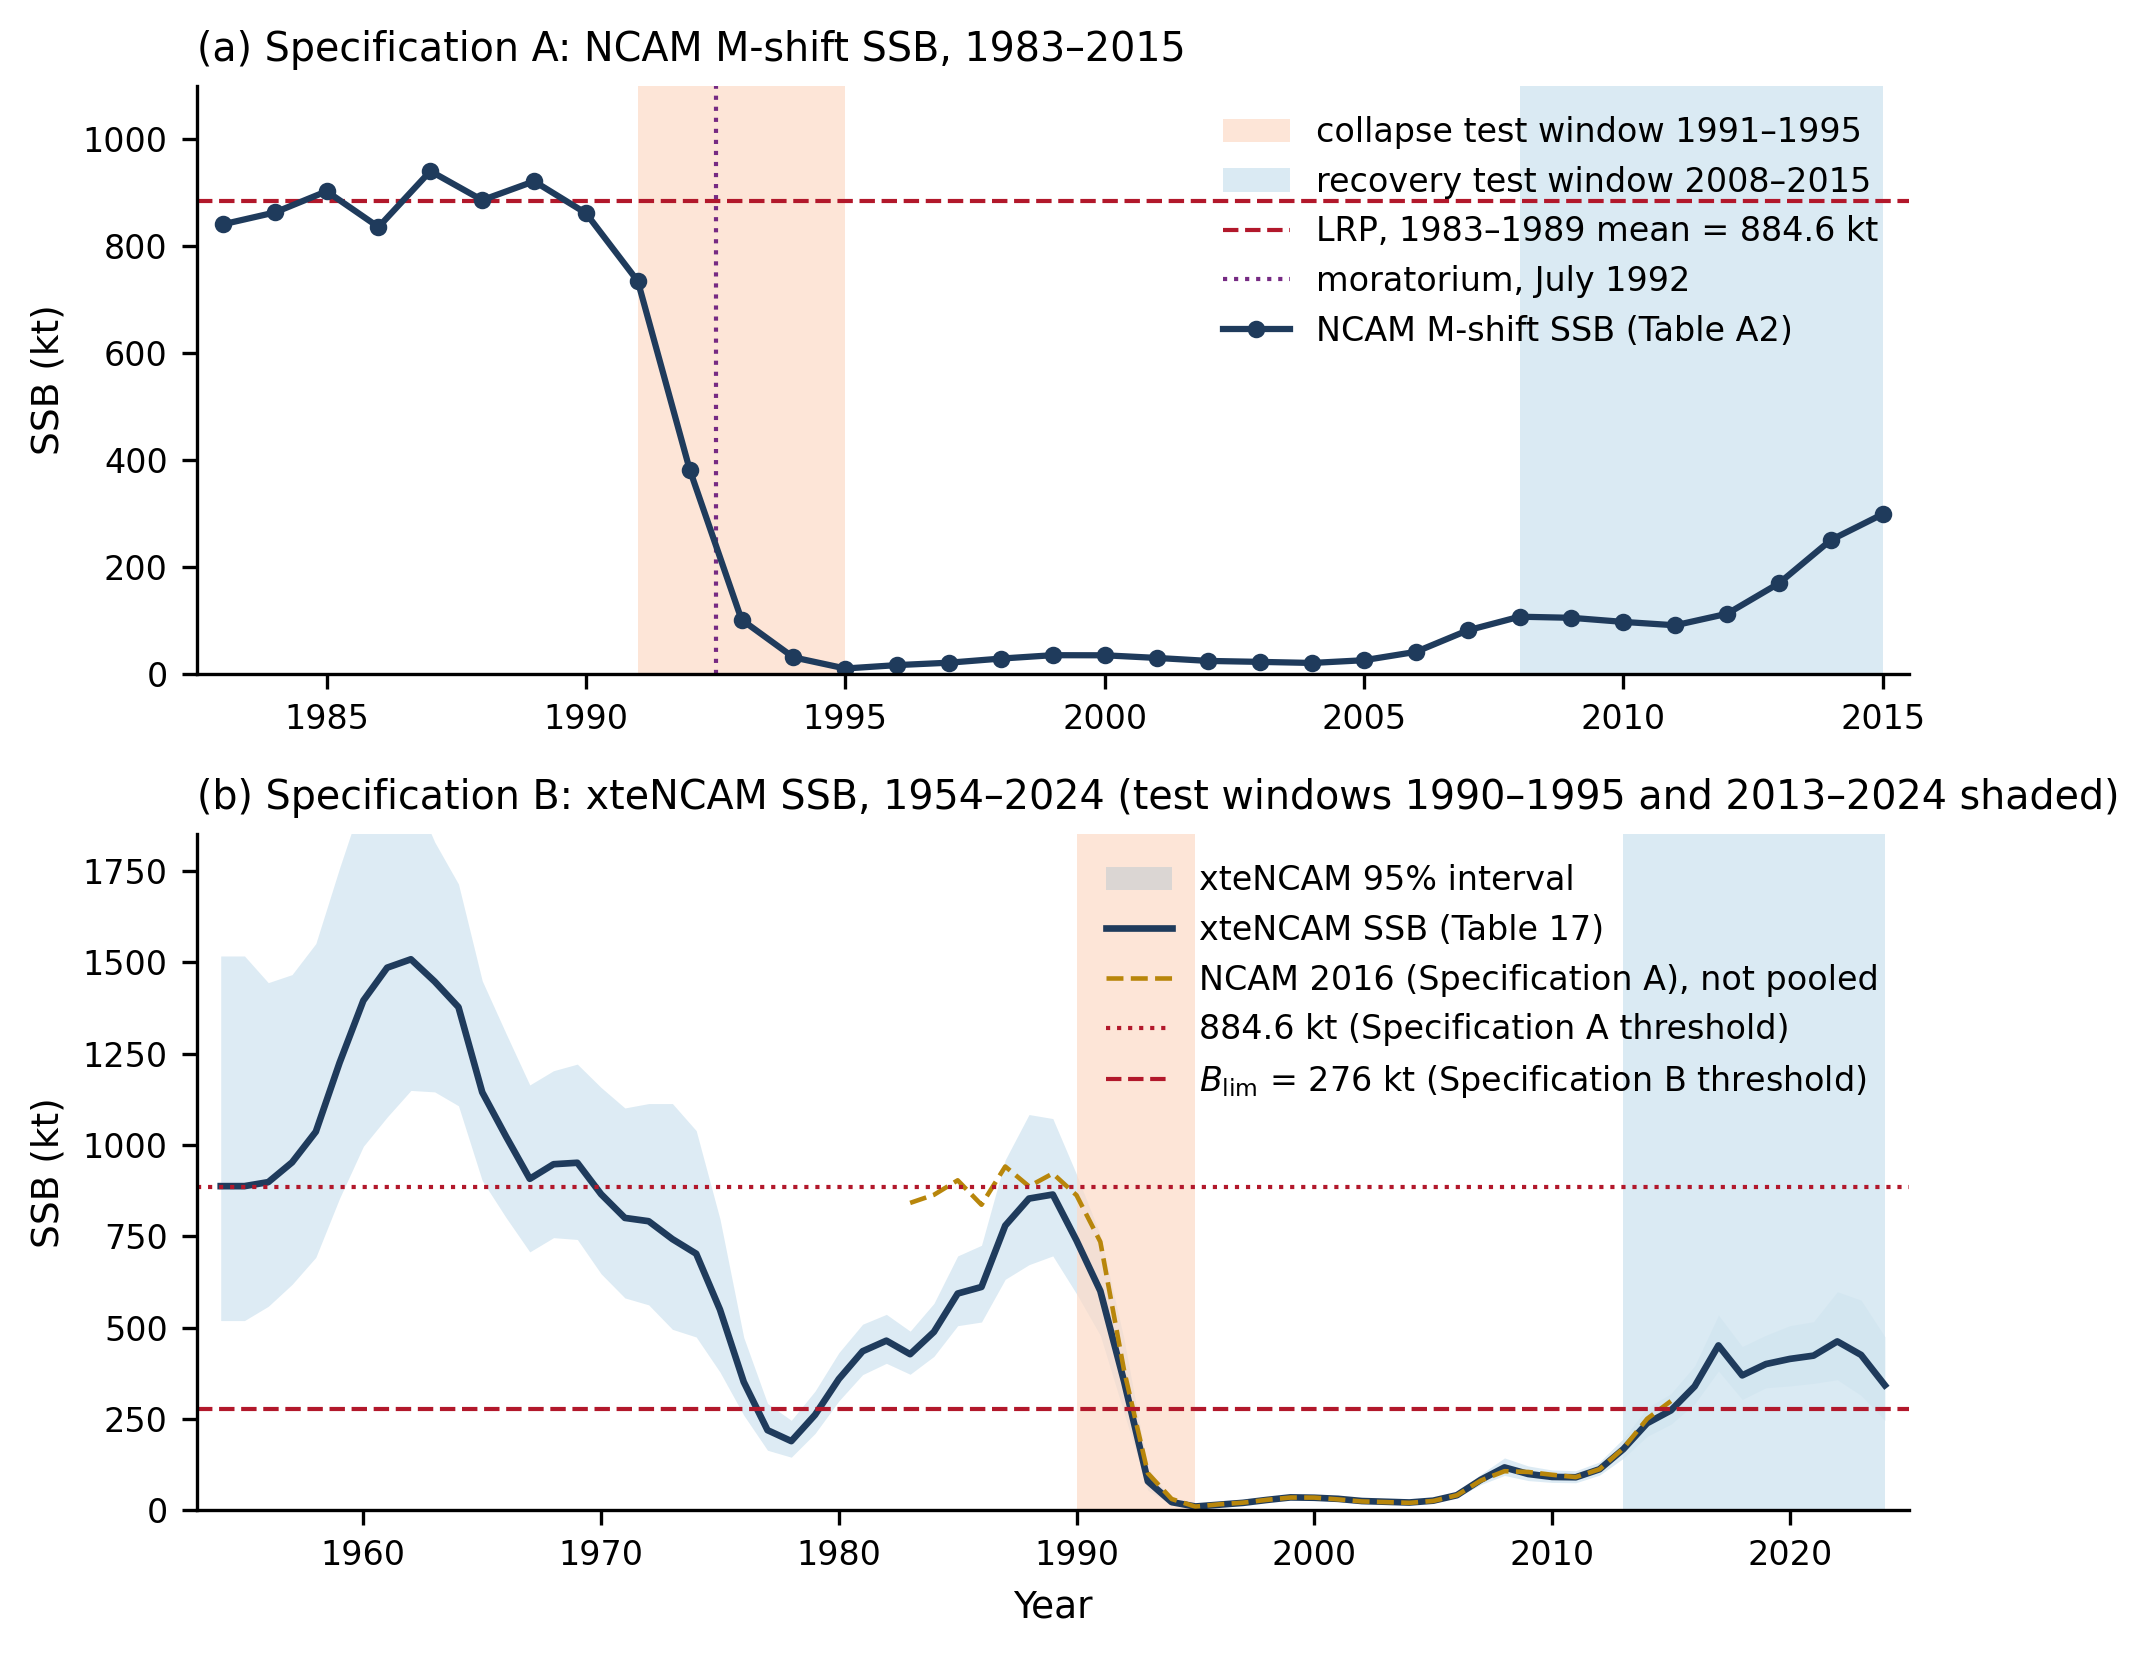
\includegraphics[width=\textwidth]{fig1_series}
\caption{The two SSB series on which the cod ladder is scored. (a) Specification A: NCAM M-shift SSB 1983--2015, with the LRP (1983--1989 mean, 884.6\,kt), the July 1992 moratorium and the two fixed test windows. (b) Specification B: xteNCAM SSB 1954--2024 with its published 95\% interval, $\Blim = 276\kt$, and the NCAM series overlaid for 1983--2015 to show the vintage difference; the series are never pooled. Shading marks the Specification B fixed test windows.}
\label{fig:series}
\end{figure}

\subsection{The surplus-production ladder}\label{sec:ladder}

All five modules are forecasters built on one difference equation.

\begin{definition}[Surplus-production map]\label{def:map}
With $S_t$ the SSB and $C_t$ the removals in year $t$,
\begin{equation}\label{eq:map}
S_{t+1} \;=\; \Spos{S_t + g(S_t) - C_t + \varepsilon_t}, \qquad
g(S) \;=\; r\,S\Bigl(1-\frac{S}{K}\Bigr)\,a(S),
\end{equation}
where $[x]_+ = \max(x,\epsilon)$ with a numerical floor $\epsilon = 10^{-3}\kt$, $r>0$ and $K>0$ are the intrinsic rate and carrying capacity of the Schaefer form \citep{Schaefer1954,Pella1969}, and $a(S)\equiv 1$ (compensatory branch) or $a(S) = (S-\sA)/(K-\sA)$ with $0<\sA<0.8K$ (depensatory branch, production negative below $\sA$). Forecasts iterate \eqref{eq:map} with $\varepsilon\equiv 0$ unless an explicit residual term is carried (M3, M4).
\end{definition}

Parameters are estimated at each origin by one-step least squares on the training transitions: $(r,K)$, and $\sA$ for the depensatory branch, minimise the mean squared difference between the observed increments $S_{j+1}-S_j$ and $g(S_j)-C_j$ over the training window (a single L-BFGS-B run from $r_0=0.3$ and $K_0=\max(1.5\max_j S_j,\,500\kt)$, with bounds $r\in[10^{-3},2]$, $K\in[\max_j S_j+10,\,5000]$, $\sA\in[0,\max_j S_j]$). The residual autocorrelation $\phi$ used by M3 and M4 is the lag-one regression coefficient of the one-step training residuals, clipped to $[-0.95,0.95]$, and the last training residual is propagated as $\phi^k$ along the horizon. The modules differ only in what they take from the catch record and the state history (Table~\ref{tab:ladder}): M1 is the autonomous Schaefer forecaster, which holds the catch at the training mean and iterates; M1b adds depensation; M2 is the stock-flow forecaster, with identical dynamics but the realised catch supplied along the horizon; M3 adds the AR(1) residual correction; M4 is M3 started from $S_{t-1}$, a lagged-start variant that tests sensitivity to the assessment lag at the origin. Fitted values at the windows and origins that matter are in SI S5; $K$ rests on its initialiser or upper bound in several fits, a point taken up in Section~\ref{sec:identification}.

\begin{table}[!htb]
\centering\small
\caption{The cod forecaster ladder. ``Comparator'' is the next-simpler module against which the module must win under (C1); M1 has no comparator within the ladder and is tested against persistence only.}
\label{tab:ladder}
\begin{tabularx}{\textwidth}{@{}l>{\raggedright\arraybackslash}p{0.23\textwidth}>{\raggedright\arraybackslash}p{0.19\textwidth}LL@{}}
\toprule
ID & Class & Free parameters & Catch in the forecast & Comparator \\
\midrule
persist & baseline & none & none & --- \\
mean & baseline & none & none & --- \\
M1 & autonomous Schaefer & $r,K$ & constant: training-mean catch & (persistence only) \\
M1b & autonomous, depensatory & $r,K,\sA$ & constant: training-mean catch & M1 \\
M2 & stock-flow & $r,K$ & realised $C_{t+1..t+h}$ supplied & M1 \\
M3 & stock-flow $+$ AR(1) residual & $r,K$; $\phi$ in a second stage & supplied & M2 \\
M4 & M3 started from $S_{t-1}$ & as M3, refitted & supplied, indexed from $t-1$ & M3 \\
\bottomrule
\end{tabularx}
\end{table}

One property of the archived runner should be stated here because it affects the one-step margins of the catch-supplied modules: estimation pairs the transition $S_t\to S_{t+1}$ with the catch $C_t$, whereas the forecast path applies $C_{t+1}$ to the same step, a one-year offset between the two conventions that was not noticed until the re-execution for the previous edition. Its effect is quantified below and in SI S14; all tabulated numbers are those of the archived runner.

\FloatBarrier
\subsection{No module is retained on either specification}\label{sec:pooled}

Table~\ref{tab:rolling} gives the pooled rolling-origin scores and Fig.~\ref{fig:gaps} the persistence margins with their bootstrap intervals. On Specification A persistence has one-step RMSE 98.0\,kt and five-year RMSE 264.7\,kt; the modules range from 114.8 to 195.6\,kt at one year and from 288.6 to 488.2\,kt at five. On Specification B persistence has 84.4 and 300.0\,kt; the modules range from 119.5 to 205.7 and from 431.9 to 1058.9\,kt. No module comes within the 5\% band of persistence at either horizon on either specification; the closest approach is M1b on Specification A, 9.0\% adrift at five years and 17.1\% at one year. Hurdle (C2) therefore fails for every module, and (C1) adds nothing that could rescue it: the only comparator margin that excludes zero is M4 against M3 on Specification A at one year, and it runs the wrong way (M4 worse by 60.9\,kt, interval $[4.4, 134.4]$). The training-mean baseline is far worse than persistence everywhere (ratios 1.7--5.4), for a reason Section~\ref{sec:synthesis} makes precise, and is not discussed further here.

\begin{table}[!htb]
\centering\small
\caption{Cod: pooled rolling-origin scores (kt). RMSE with, in parentheses, the ratio to origin-matched persistence; MAE alongside. Specification A: coarse-regime catch, origins 1990--2014 ($n=25$, $h=1$) and 1990--2010 ($n=21$, $h=5$). Specification B: origins 1965--2023 ($n=59$) and 1965--2019 ($n=55$). A module is retained under Protocol C only if its ratio is below 0.95 at both horizons and it also beats its comparator (Table~\ref{tab:ladder}); none is.}
\label{tab:rolling}
\resizebox{\textwidth}{!}{%
\begin{tabular}{@{}lrrrrrrrr@{}}
\toprule
 & \multicolumn{4}{c}{Specification A} & \multicolumn{4}{c}{Specification B} \\
\cmidrule(lr){2-5}\cmidrule(lr){6-9}
 & \multicolumn{2}{c}{$h=1$} & \multicolumn{2}{c}{$h=5$} & \multicolumn{2}{c}{$h=1$} & \multicolumn{2}{c}{$h=5$} \\
Forecaster & RMSE & MAE & RMSE & MAE & RMSE & MAE & RMSE & MAE \\
\midrule
persistence & 98.0 (1.00) & 48.1 & 264.7 (1.00) & 137.2 & 84.4 (1.00) & 58.7 & 300.0 (1.00) & 217.3 \\
training mean & 423.6 (4.32) & 375.2 & 507.4 (1.92) & 447.8 & 458.1 (5.43) & 397.3 & 521.6 (1.74) & 456.8 \\
M1 autonomous & 120.5 (1.23) & 79.7 & 288.7 (1.09) & 158.2 & 119.5 (1.42) & 93.7 & 431.9 (1.44) & 335.7 \\
M1b depensatory & 114.8 (1.17) & 79.6 & 288.6 (1.09) & 158.2 & 151.6 (1.80) & 117.6 & 445.5 (1.49) & 344.1 \\
M2 stock-flow & 144.1 (1.47) & 60.6 & 398.2 (1.50) & 193.5 & 166.0 (1.97) & 106.2 & 1058.9 (3.53) & 758.7 \\
M3 AR residual & 134.6 (1.37) & 52.9 & 366.4 (1.38) & 183.2 & 126.7 (1.50) & 80.2 & 930.1 (3.10) & 650.8 \\
M4 lagged start & 195.6 (1.99) & 82.2 & 488.2 (1.84) & 223.6 & 205.7 (2.44) & 127.8 & 1030.7 (3.44) & 740.2 \\
\bottomrule
\end{tabular}}
\end{table}

\begin{figure}[!htb]
\centering
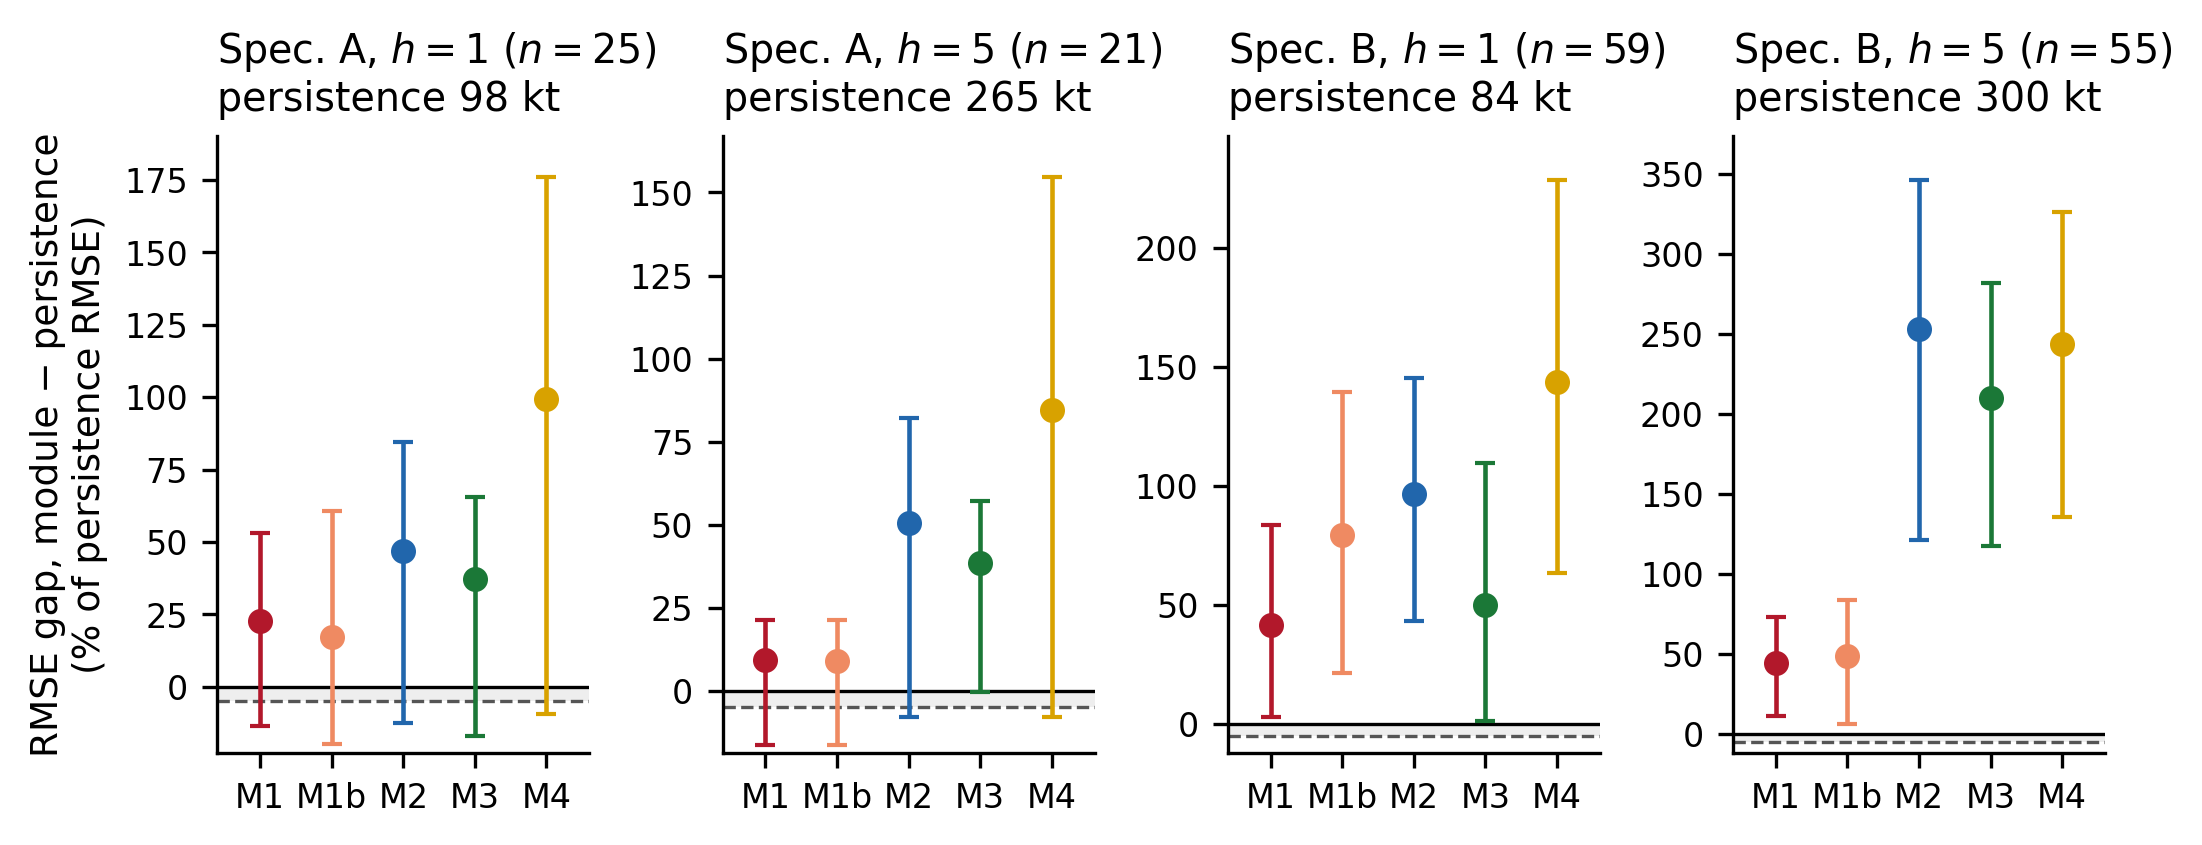
\includegraphics[width=\textwidth]{fig2_gaps}
\caption{Cod: persistence margins, RMSE of each module minus RMSE of origin-matched persistence as a percentage of the persistence RMSE, with 95\% paired moving-block bootstrap intervals (block $\max(h,3)$, 20\,000 replicates). The dashed line is the 5\% tie band; retention under (C2) requires the point estimate to lie below it. On Specification A every interval contains zero; on Specification B every interval lies above zero at the block length of the archived layer.}
\label{fig:gaps}
\end{figure}

The two specifications differ in what can be said about the margins. On Specification A every persistence margin has a bootstrap interval containing zero (M1 at one year: $+22.5\kt$, $[-13.4, +52.2]$, $p=0.19$; M3: $+36.6$, $[-16.8, +64.2]$, $p=0.93$), so the data do not show that the modules are worse than persistence, only that they are not demonstrably better; the five-year M3 margin is the nearest to significance ($+101.6$, $[-0.8, +151.4]$, $p=0.08$). On Specification B every persistence margin excludes zero at the archived block length (M1 at one year: $+35.0$, $[+2.7, +70.8]$, $p=0.03$; M3: $+42.3$, $[+1.0, +92.5]$, $p=0.04$; all five-year margins $p\le 0.02$). The M3 one-step margin on B is the only interval whose classification depends on the block length (SI S3). Re-running the catch-supplied modules with the consistent catch-timing convention, a sensitivity outside the archived protocol (SI S14), lowers their one-step RMSE by 20--75\,kt and their five-year RMSE by up to 16\%; M3 then stands 7\% above persistence at one year on A and 12\% on B, still outside the band, and every five-year margin remains far outside it. The verdict does not depend on the convention; the size of the one-step deficit does. The MAE columns show that the one-step deficit is concentrated in a few large errors: on Specification A the M3 MAE is 10\% above persistence where its RMSE is 37\% above. Where those errors sit is the next question.

\FloatBarrier
\subsection{Where the deficit arises}\label{sec:periods}

Protocol C is applied to the pooled score, but pooling averages over regimes that the stock did not average over. Table~\ref{tab:periods} splits the one-step rolling errors into the periods visible in Fig.~\ref{fig:series} and Fig.~\ref{fig:period} shows the per-origin errors behind it; the decomposition is post hoc and is reported as a description of the data, not as a second test. Three features emerge.

\begin{table}[!htb]
\centering\small
\caption{Cod: one-step rolling-origin RMSE (kt) by period of the forecast origin, with origin-matched persistence. Superscripts give the number of origins at which the module's forecast sits at the numerical floor ($<0.01\kt$), i.e.\ forecasts extinction; its absolute error is then the observed SSB. Bracketed values are paired bootstrap intervals for the module$-$persistence gap in kt (block 3, 20\,000 replicates; not shown for bands with $n<11$). Five-year values and the annual-landings pass are in SI S4.}
\label{tab:periods}
\resizebox{\textwidth}{!}{%
\begin{tabular}{@{}llrrrrrrr@{}}
\toprule
Spec. & Origins & $n$ & persist & M1 & M1b & M2 & M3 & M4 \\
\midrule
A & 1990--1995 (collapse) & 6 & 193.6 & 208.8$^{3}$ & 186.4$^{4}$ & 292.0 & 273.2$^{3}$ & 397.3 \\
A & 1996--2012 (low biomass) & 17 & 19.6 & 64.8$^{12}$ & 69.7$^{13}$ & 17.2 & 14.7 & 19.4 \\
A & 2013--2014 (early rebuild) & 2 & 66.7 & 122.7 & 138.9 & 32.4 & 28.6 & 38.1 \\
A & 1996--2014 pooled & 19 & 28.5 & 73.1 & 79.8 & 19.4 & 16.7 & 22.1 \\
 & \quad gap vs.\ persistence & & & $+44.6$ & $+51.3$ & $-9.1$ & $-11.8$ & $-6.4$ \\
 & \quad 95\% interval & & & $[+29, +60]$ & $[+29, +69]$ & $[-17, +7]$ & $[-20, +3]$ & $[-14, +9]$ \\
\midrule
B & 1965--1990 (fished, pre-collapse) & 26 & 94.7 & 142.4$^{2}$ & 186.4$^{3}$ & 184.2 & 166.3 & 260.6 \\
B & 1991--1995 (collapse) & 5 & 167.0 & 126.8$^{3}$ & 66.6$^{3}$ & 299.8 & 154.8$^{3}$ & 321.6$^{1}$ \\
B & 1996--2012 (low biomass) & 17 & 20.7 & 75.0$^{17}$ & 75.0$^{17}$ & 26.3 & 19.7 & 24.0 \\
B & 2013--2023 (rebuild) & 11 & 61.0 & 112.3 & 174.5$^{1}$ & 160.5 & 96.4 & 136.3 \\
B & 1996--2023 pooled & 28 & 41.5 & 91.5 & 124.0 & 102.7 & 62.3 & 87.4 \\
 & \quad gap vs.\ persistence & & & $+50.0$ & $+82.5$ & $+61.2$ & $+20.9$ & $+46.0$ \\
 & \quad 95\% interval & & & $[+26, +79]$ & $[+53, +118]$ & $[-2, +93]$ & $[-11, +47]$ & $[-5, +73]$ \\
\bottomrule
\end{tabular}}
\end{table}

\begin{figure}[!htb]
\centering
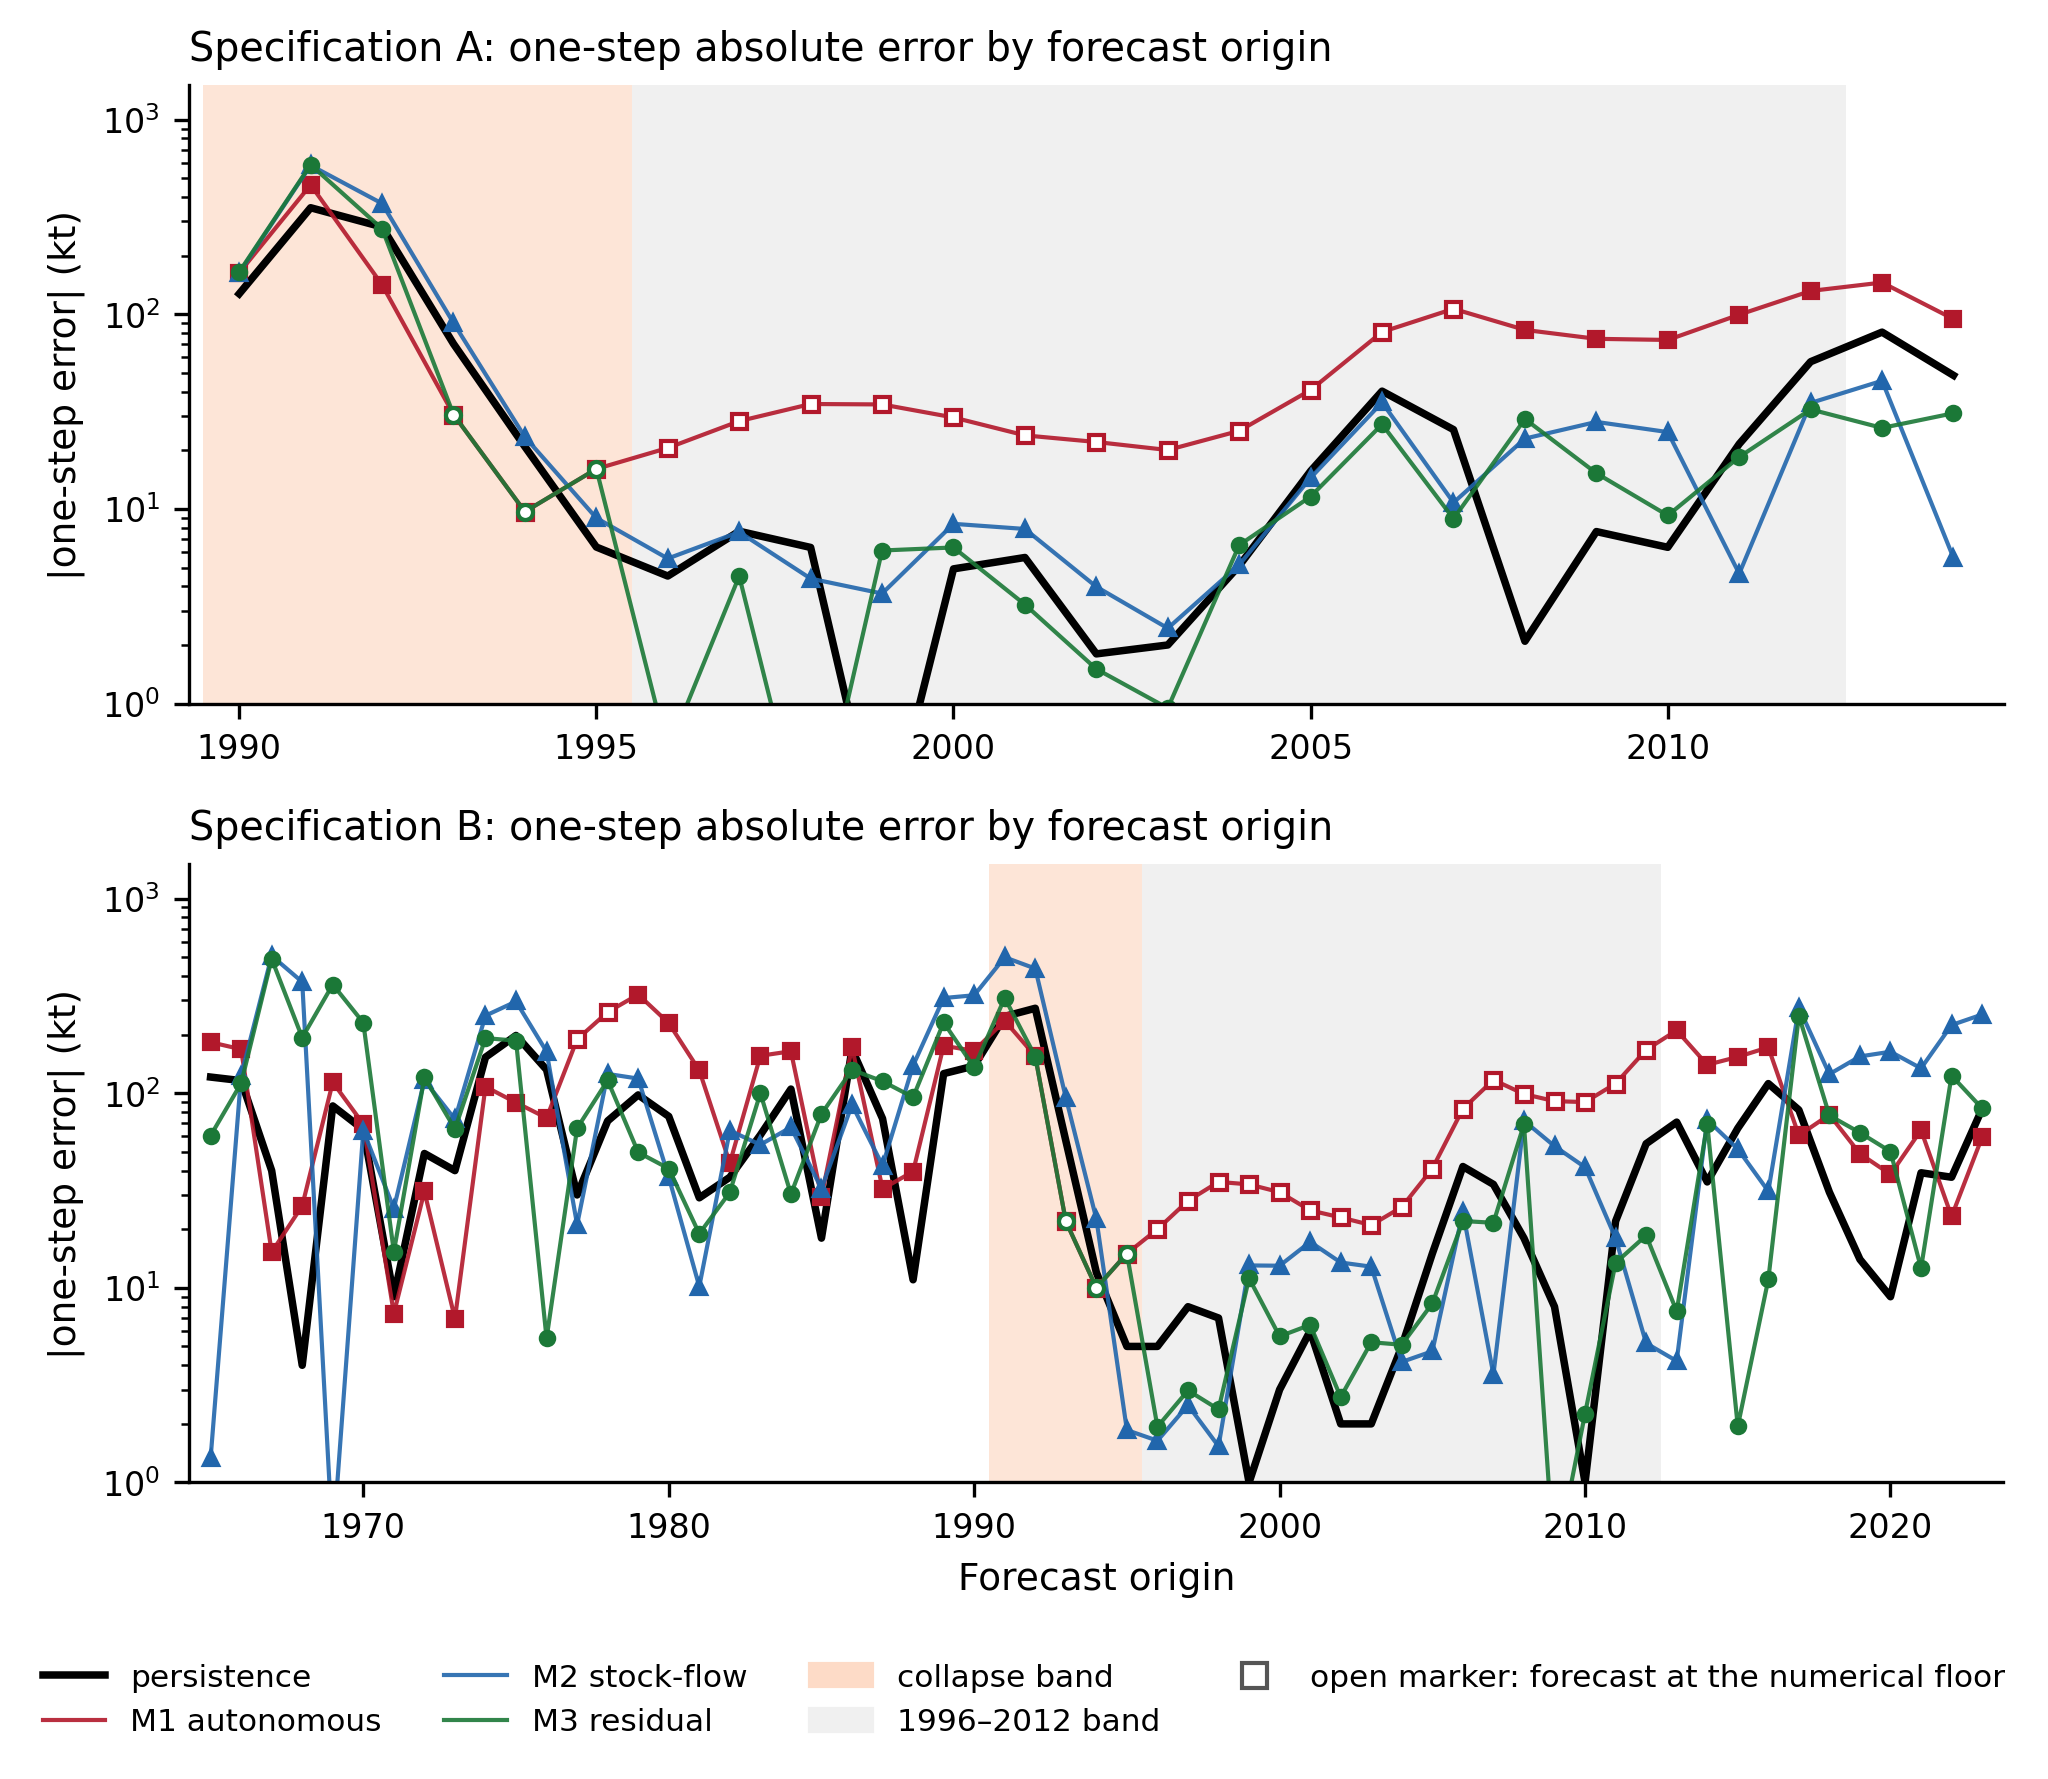
\includegraphics[width=\textwidth]{fig4_period}
\caption{Cod: one-step absolute error by forecast origin (log scale, floored at 1\,kt for display) for persistence, M1, M2 and M3 on (top) Specification A and (bottom) Specification B. Shading marks the collapse band and the 1996--2012 low-biomass band. Open markers are forecasts at the numerical floor: at those origins M1's error is simply the observed SSB, which is why its curve traces the stock trajectory through 1996--2012 on both panels.}
\label{fig:period}
\end{figure}

First, the pooled deficit is carried by the collapse band. On Specification A the six origins 1990--1995 contribute 94\% of the pooled one-step sum of squared persistence errors and 63--99\% of each module's; every forecaster is wrong by 130--590\,kt at the 1991 origin and by 140--710\,kt at the 1992 origin, because every forecaster, including persistence, extrapolates a state that is about to be removed. On Specification B the 26 fished pre-collapse origins add a second source of deficit: between 1965 and 1990 the catch-supplied modules are worse than persistence by 70--170\,kt, as a stock-flow model fitted to a series with 200--800\,kt removals mis-times the large swings of the 1960s and 1970s.

Second, the apparent collapse-band wins of M1, M1b and M3 on Specification B, and of M1b on A, are not forecasts of the collapse. At the 1993--1995 origins these modules forecast the floor: their training-mean catch (317--333\,kt on B, 177--208\,kt on A) exceeds the production of a stock of 10--100\,kt by an order of magnitude, so the map drives the state to $10^{-3}\kt$ in one step and the absolute error equals the observed value, which is small only because the stock was nearly gone. A floor forecast is a correct sign with no magnitude; it is credited by RMSE and should not be read as skill.

Third, the autonomous modules forecast extinction at every post-collapse origin, and the catch-supplied modules have one-step skill in the low-biomass regime on one specification only. Between 1996 and 2012 M1 and M1b sit at the floor at 17 of 17 origins on Specification B and at 12--13 of 17 on A; their RMSE in that band, 65--75\,kt against 20\,kt for persistence, is the root mean square of the observed SSB. Training-mean catch is a plug, not an estimate, and after a collapse it is a plug an order of magnitude above sustainable removals. In the same band M2, M3 and M4 forecast within 15--26\,kt, and on Specification A they beat persistence: pooling 1996--2014, M3 has one-step RMSE 16.7 against 28.5\,kt, a gap of $-11.8\kt$ ($-41\%$) with interval $[-20.5,+3.3]$, $p=0.19$. The intervals contain zero and the bands were chosen after the fact, but the point estimates are the right sign and the right order to be the residual signal that a catch-supplied production model should carry when the catch is small and the stock is far below $K$. On Specification B the same bands give the opposite answer: post-1995 every module is worse than persistence at one year and at five years by factors of 2--6, because the 2013--2023 rebuild, which Specification A does not contain, is forecast by the stock-flow modules as a rise several hundred kilotonnes above what occurred. The low-biomass skill does not transfer across the two series.

\FloatBarrier
\subsection{Why the collapse cannot be forecast from inside the class}\label{sec:identification}

The fixed windows (SI S4) show the behaviour the pooled scores summarise: from the 1983--1990 training window, in which SSB varied between 835 and 942\,kt, every module forecasts continuation, the autonomous modules holding the stock at the fitted equilibrium of 888.6\,kt and the catch-supplied modules, told that removals fall from 240 to 120 to 5\,kt, forecasting growth to about 1050\,kt by 1993 while the observed path falls from 862 to 9.7\,kt. This has a structural explanation that does not depend on the fitted values. Write $F_C(S) = \Spos{S + g(S) - C}$ for the deterministic map at catch $C$.

\begin{proposition}\label{prop:repeller}
Let $g$ be continuous with $g(0)=0$, let $C>0$, and let $S_-(C) = \inf\{S>0 : g(S)\ge C\}$, with $S_-(C)=\infty$ if the set is empty.
\begin{enumerate}[label=(\roman*),leftmargin=2.2em,itemsep=1pt]
\item Every trajectory of $F_C$ started in $[0,S_-(C))$ is nonincreasing and remains in $[0,S_-(C))$; on any interval on which $g \ge C$, $F_C(S)\ge S$, so a trajectory cannot decline in one step from a state in that interval.
\item A one-step decline larger than the removals, $S_{t+1} < S_t - C_t$, requires $g(S_t) < 0$. On the compensatory branch this is impossible for $0\le S_t\le K$, whatever $(r,K)$; on the depensatory branch it requires $S_t < \sA$.
\end{enumerate}
\end{proposition}

The proof is in \ref{app:proofs}. For the Schaefer branch with $4C\le rK$, $S_-(C) = \tfrac{K}{2}\bigl(1-\sqrt{1-4C/(rK)}\bigr)$ is the lower, unstable equilibrium and $S_+(C)=K-S_-(C)$ the upper, stable one, with $g\ge C$ between them; for $4C>rK$ production never reaches the catch and every trajectory declines to the floor. Three consequences follow. First, the lower equilibrium is generated by the catch: it vanishes as $C\to 0$ and it exists on the compensatory branch with no depensation term at all, so a threshold below which the autonomous map declines is a statement about sustained removals, not about the biology of small populations. Second, the 1990 state, 862\,kt, lies between $S_-=144$ and $S_+=888.6\kt$ for the fitted map under 240\,kt, so by (i) the autonomous forecast cannot decline at all; it rises to the attractor, which is locally stable ($F_C'(S_+)=-0.39$). Third, and independently of any fit, the 1991, 1992 and 1993 transitions are declines larger than the recorded catch: apparent net production $S_{t+1}-S_t+C_t$ is $-113$, $-161$ and $-66\kt$ under the coarse regime and $-181$, $-240$ and $-59\kt$ under annual landings (Fig.~\ref{fig:production}). By (ii) no parameter value of the compensatory branch, and no catch-supplied module built on it, can reproduce these steps; the depensatory branch can do so only with a threshold $\sA$ above 735\,kt, which no fit approaches. The collapse lies outside the model class at the recorded catch. The assessment model itself accommodates these years through under-reported catch and an elevated natural mortality \citep{Cadigan2016}; a forecaster that takes the catch record as given cannot, and a forecaster that is told the catch is falling to 5\,kt forecasts growth.

\begin{figure}[!htb]
\centering
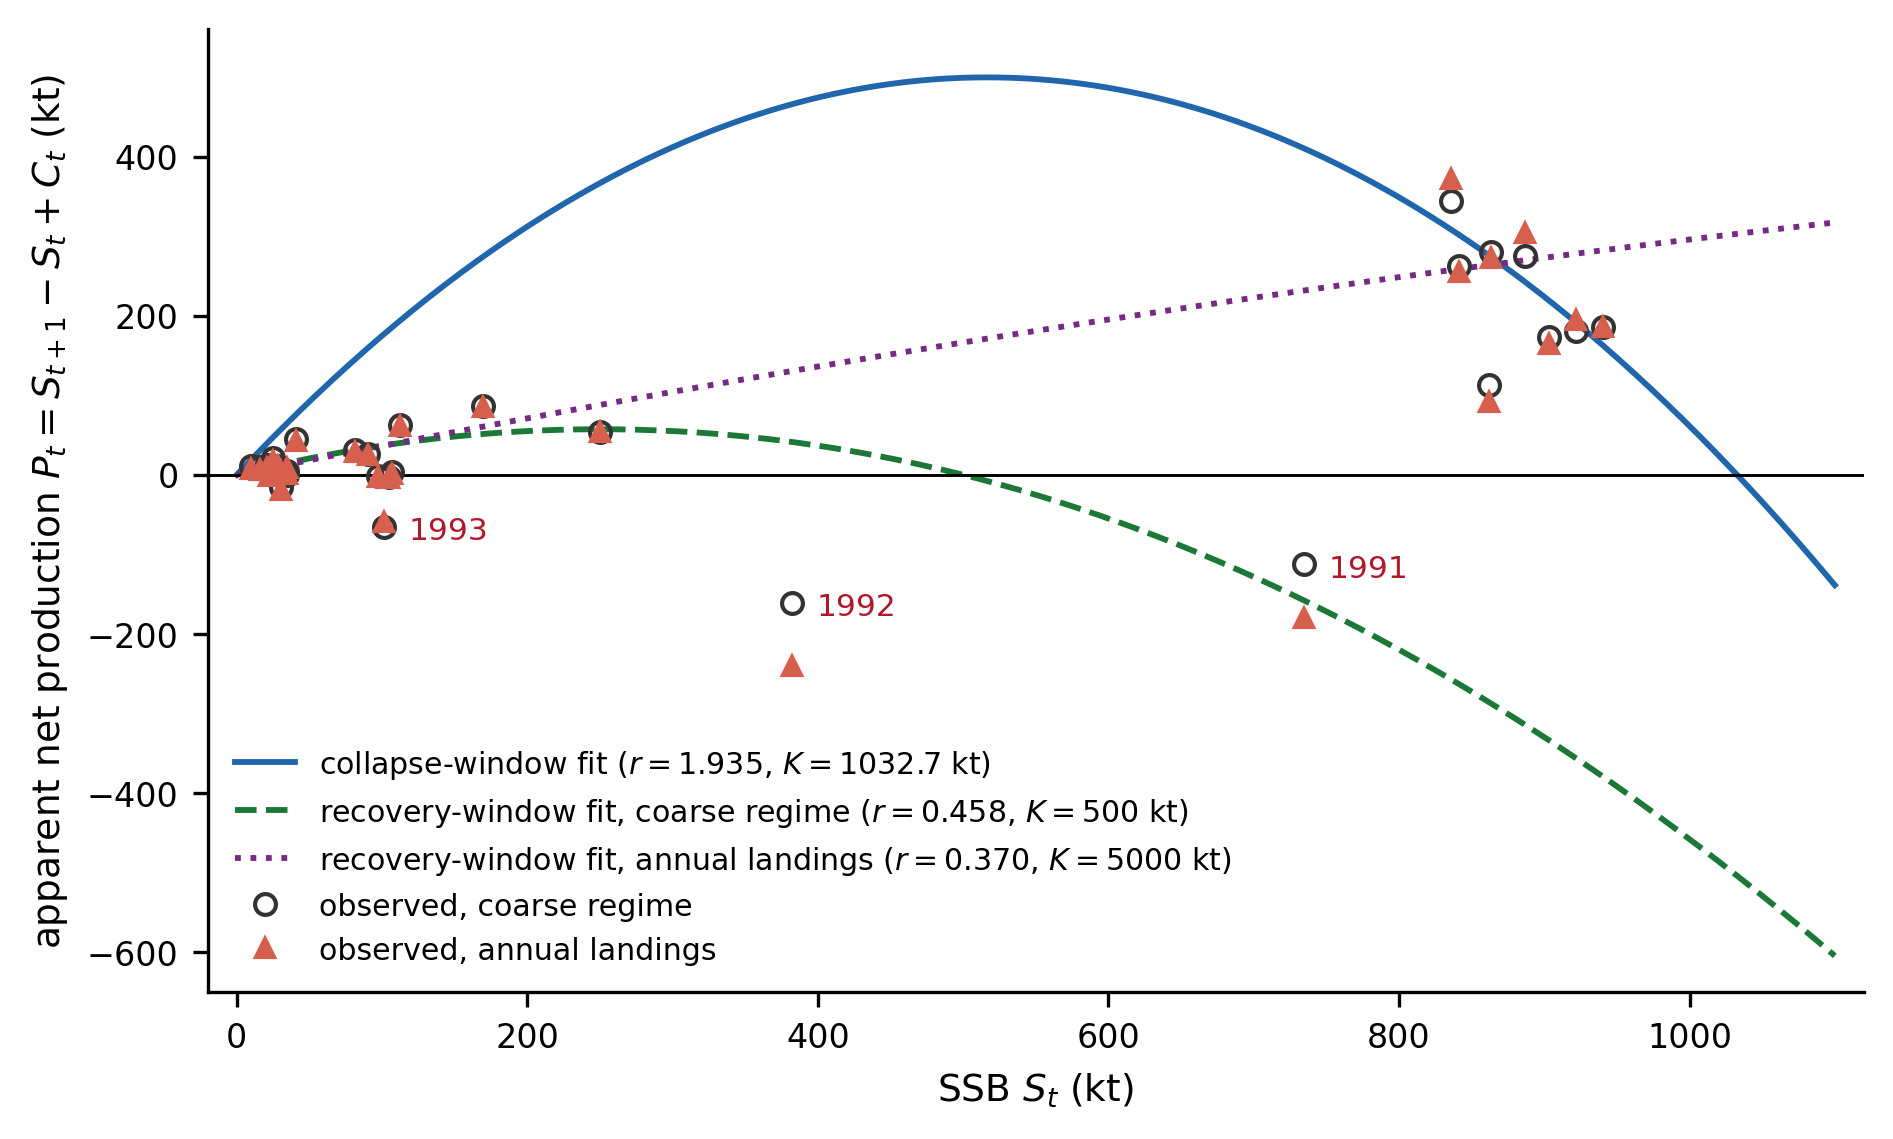
\includegraphics[width=0.9\textwidth]{fig5_production}
\caption{Cod: apparent net production $S_{t+1}-S_t+C_t$ against $S_t$ on Specification A, with the collapse-window fit ($r=1.935$, $K=1032.7$; maximum $rK/4=500\kt$ at $S=516$) and the two recovery-window fits. Under 240\,kt of removals the collapse-window map has its repeller at $S_-=144\kt$ and its attractor at $S_+=889\kt$. The 1991--1993 transitions lie below every nonnegative production curve: the stock lost more biomass than the recorded catch removed. The recovery-window fits are nearly linear through the low-biomass points, with $K$ at its initialiser (500\,kt, coarse regime) or at its upper bound (5000\,kt, annual landings).}
\label{fig:production}
\end{figure}

The depensatory branch does not change this. In the fixed windows, which exclude the collapse transitions from training, M1b's $\sA$ estimate sits at its lower bound of zero, and the profile of the objective over $\sA$ changes by 3--7\% across its whole range (SI S5). In rolling fits whose training window contains the collapse, the estimate jumps to 585--734\,kt on Specification A at every origin from 1992 to 2010 and falls back to 5\,kt from 2011, while on Specification B it stays at zero throughout (SI S5). A depensation parameter that is zero, 700\,kt or 5\,kt depending on the window is not an estimate of an Allee threshold; it is the branch's only means of absorbing transitions the class cannot otherwise represent. Whether depensation has delayed the recovery \citep{Shelton1999,Hutchings1996,Rose2026} is therefore not a question this test can answer, and the usual difficulty of detecting depensation from assessment series \citep{Myers1995,Liermann1997} is compounded by a collapse that the class attributes to it by default. The compensatory fits are weakly identified as well: $K$ rests at its 5000-kt bound at 23 of the 25 Specification A origins from 1992 onward, so the post-collapse stock-flow forecaster is in effect linear, $S_{t+1}\approx(1+r)S_t-C$ with $r\approx0.25$ (A) and $0.50$ (B), the familiar outcome of fitting a production model to a series with little contrast \citep{HilbornWalters1992,LudwigWalters1985,Polacheck1993}. That linear growth term is the whole of the low-biomass skill reported in Section~\ref{sec:periods}.

\FloatBarrier
\subsection{Operating characteristics of Protocol C}\label{sec:operating}

Fig.~\ref{fig:operating} reports retention frequencies from 200 replicates per cell under the seven data-generating processes of Section~\ref{sec:power}. For the collapse-window autonomous Schaefer truth (D1), the rule retains M1 in 97.5\% and 95.0\% of replicates at the two noise levels; at recovery-window parameters (D2), power is 66.0\% and 11.0\%. For the stock-flow truth (D3), true-M2 power is 10.5\% and 13.0\%; for the depensatory truth (D4), true-M1b power is 0.0\% and 1.5\%. Truth-specific power is not the same as selecting any member of the ladder: under D3, some module is retained in 52.5\% and 61.0\% of replicates, and under D4 in 30.5\% and 5.5\%, respectively, so the low true-module rates do not imply that the rule usually selects nothing. Under the persistence-true null (D5), any-module false retention is 2.5\% and 7.5\%, both point estimates below the pre-declared 10\% bar. The two processes outside the class exceed that bar substantially: a drifting-productivity truth (D6) yields any-module retention in 72.0\% and 77.0\% of replicates, and a smooth path observed with error (D7) in 97.0\% and 95.0\%, mostly M1. The rule is therefore specific against this persistence null under the stated design, not against the presence of structure of another kind; it detects that something beyond persistence may be present, not that the retained module is that something. Cell-specific Wilson intervals are in SI Table~S16; they quantify Monte Carlo uncertainty only. The Protocol C reference row in SI S8 is recomputed from the completed v68 archive; earlier alternative-rule summaries remain as reported. Their calculation code or complete formula was not located for this edition, so those alternatives are not independently reproduced and do not inform the present primary-rule conclusions.

\begin{figure}[!htb]
\centering
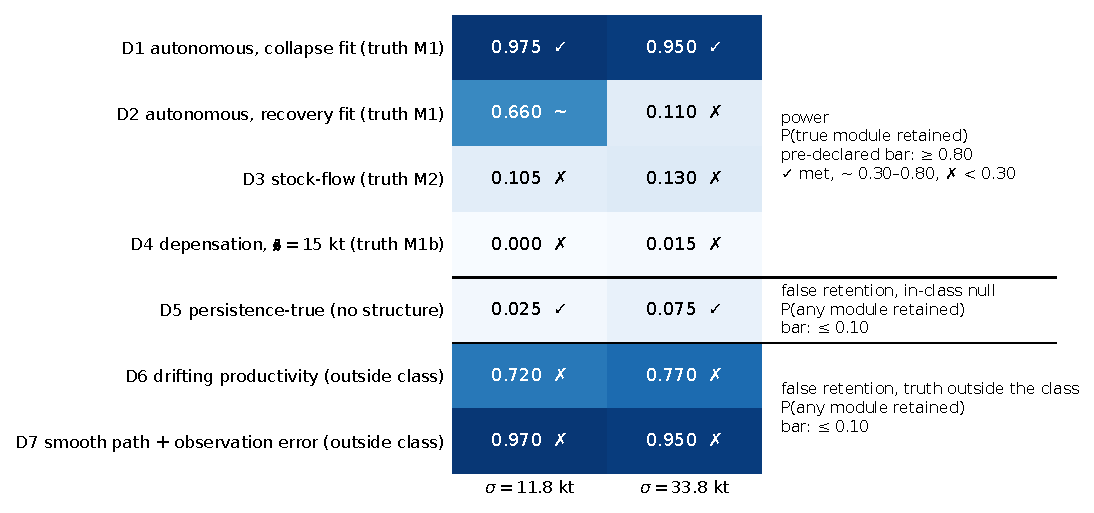
\includegraphics[width=\textwidth]{fig6_operating}
\caption{Cod: point estimates of Protocol C retention frequencies under seven data-generating processes (200 replicates per cell, two process-noise levels; Specification A design). D1--D4 show retention of the truth-matching module (power; pre-declared bar 0.80); D5--D7 show retention of any module (false retention; bar 0.10). Cell-specific 95\% Wilson intervals, reflecting Monte Carlo uncertainty only, are reported in SI Table~S16.}
\label{fig:operating}
\end{figure}

\FloatBarrier
\subsection{Variant passes and the years after 2015}\label{sec:verdict}

Four variant passes were added after the primary pass and declared in order (SI S1, S4), each scored against persistence recomputed on its own origin set: annual landings in place of the coarse regime (M2 160.4, M3 153.6, M4 206.3\,kt at one year against 98.0 for persistence); a survey-scaled start value (128.1 and 331.0\,kt); a two-regime intrinsic rate with a 1991 break at the capelin collapse \citep{Buren2014,DFO2024b} (153.8 and 334.0\,kt on A; 146.8 and 894.4 on B); and a capelin acoustic-index multiplier on the years with an acoustic estimate \citep{Murphy2025,NAFC2025} (150.0 and 262.3\,kt on A against 96.6 and 193.0 for persistence on the reduced set). No variant comes within the band at either horizon.

Specification A ends in 2015, and the continuation of the same assessment family is published in the RAM Legacy database \citep[v4.66, stock COD2J3KL;][]{Ricard2012}, with xteNCAM reading the same years independently (SI S11). The outcome window is an increase regime: every year 2016--2021 lies above its 2015 origin in both vintages, so it contains no event of the kind the collapse test probes, and persistence from the 2015 origin errs low throughout (RMSE 133.3\,kt on the RAM vintage). The two vintages agree on the outcome years to within 1--26\,kt while on the historical overlap they do not (the Table A2 vintage runs 24.7\,kt above the RAM vintage on average over 1983--2015, with a maximum difference of 131\,kt), so that the LRP defined as the 1983--1989 mean is 884.6\,kt on one vintage and 790.0\,kt on the other; the two thresholds classify the same xteNCAM file differently in 29 of 71 years; and the 2023 framework revision moved the reported zone from critical to cautious without a change in the stock \citep{DFO2024a,Regular2025}. Over the same period the observing system lapsed: partial fall-survey coverage in 2021 and 2022 left the leading indicator uncomputable, no typical assessment update was possible in 2022 or 2023, and the survey vessel was condemned (SI S12). None of this touches the RMSE comparison, which never uses a threshold; all of it bears on the verdict any forecast is scored against, and after 2015 the reference-point and observation layers moved more than forecast skill did.

\subsection{Reading the cod verdict}\label{sec:codreading}

A negative verdict from a scored test carries the weight of the test's power, and Section~\ref{sec:operating} lets that weight be assigned per module. For M1 the verdict is strong: at the collapse-window parameters the rule retains a true autonomous Schaefer module in 97.5\% and 95.0\% of replicates, so its non-retention on both empirical specifications, with a persistence margin that excludes zero on Specification B, is evidence against an autonomous production model driven by mean historical catch as a description of this stock's year-to-year SSB transitions. For M2, M3 and M4 the verdict is weak: against the D3 stock-flow process the full rule retains true M2 in 10.5\% and 13.0\% of replicates. The persistence-only hurdle is passed in 12.0\% and 54.0\%; the comparator then removes 12.5\% and 75.9\% of those survivors, respectively. Thus low full-rule power, especially at the higher noise level, reflects both difficulty clearing persistence and attrition at the comparator gate; it is not evidence that catch-supplied structure is absent. The low-biomass skill on Specification A is consistent with that limited reading, and its failure to extrapolate is evidence that what the modules carry is a short-memory growth term. For M1b the verdict is not about depensation at all: the parameter it adds is unidentified, and the test could not have retained a true depensatory module. Three features of assessment output make persistence a demanding benchmark on an assessed state, and they are the reason this paper scores on the state: the series is a retrospective estimate smoothed by the assessment's process-error structure, so the last value is an efficient summary of the recent past; the forecaster is fitted to the same smoothed series and learns slow dynamics, then adds a parametric shape and a catch plug the series does not demand; and the quantity that moves the series most, the collapse, is one that no member of the class can reproduce at the recorded catch, so the model carries the full persistence error there and adds its own. Hindcast cross-validation on the fitted index \citep{Kell2016,Kell2021,Carvalho2021} answers whether the assessment predicts its own data, which is a different and easier question than whether its dynamics predict next year's biomass.
\FloatBarrier
\section{System II: Edwards Aquifer, index well J-17}\label{sec:edwards}

\subsection{Data and specification}\label{sec:edw_data}

The predictand is the calendar-year mean of daily-high elevation at well J-17 (TWDB 6837203, EAA AY-68-37-203), the index well of the San Antonio Pool of the Edwards (Balcones Fault Zone) Aquifer, for 1934--2023 (Table~\ref{tab:edwspec}, Fig.~\ref{fig:edwseries}). Three hydrological objects are read off this one number and should be kept apart: the head is observed at an access point; it indexes a store of water, which is the resource; and the store is replenished and drawn by fluxes, which are the flow. The one-pool water balance closes this loop approximately, in the increment-structure sense used throughout: head change equals weighted fluxes plus a linear drain. It is not a closed mass balance. Annual means use all available daily highs; no year falls below the 240-observation floor (minimum $n=242$ in 1939); missing days are not interpolated; the published pre-continuous composite is used as issued; and the 2023 values carry provisional status. Recharge $R$ is USGS total San Antonio-area recharge ($10^3$ acre-ft\,yr$^{-1}$), estimated by the stream-loss method of \citet{Puente1978} and constructed independently of J-17 \citep{UmphresChoi2025}; pumpage $P$ is well discharge from Edwards Aquifer Authority Table 1 \citep{EAA2024}. Both are constructed fluxes, not observations of J-17, and total-area values mix the San Antonio and Uvalde pools. Spring discharge is stored and not used as a driver. Climate predictors, used only by the climate-informed variants, are September--November Ni\~no~3.4 (HadISST) and calendar-year precipitation in Texas climate divisions 06 and 07 (NCEI nClimDiv). Two thresholds frame the series without entering any forecast: the Edwards Aquifer Authority's Stage~I line (10-day mean J-17 below 660\,ft, a 2007 institutional rule) and the physical level near 618\,ft at which Comal Springs approaches cessation (1956 daily minimum 612.51\,ft). The annual mean is below 660\,ft in 31 of 90 years; the daily minimum is below 618\,ft in one (1956).

\begin{table}[!htb]
\centering\small
\caption{The J-17 specification. D = data, E = empirical construct, M = model, N = normative threshold. The predictand is a measured well series, not a storage reconstruction, a numerical-model inversion, the J-27 Uvalde index or spring discharge.}
\label{tab:edwspec}
\begin{tabularx}{\textwidth}{@{}>{\raggedright\arraybackslash}p{0.24\textwidth}Lc@{}}
\toprule
Field & Contents & Type \\
\midrule
System & Edwards Aquifer, San Antonio Pool, indexed by J-17 & D \\
Predictand $H_t$ & calendar-year mean of daily-high J-17 elevation (ft AMSL), 1934--2023 (90 years) & D \\
Drivers & recharge $R_t$ (USGS, stream-loss method); pumpage $P_t$ (EAA Table 1) & D/E \\
Physical threshold & head at which Comal Springs does not cease ($\approx$618\,ft) & N/E \\
Institutional threshold & EAA Stage I, 10-day mean $<660$\,ft (in force after 2007); the annual-mean indicator is a coarse proxy & N \\
Disturbance & recharge pulses; unmodelled karst; Uvalde--San Antonio exchange & M \\
Service series & USGS 08168710 Comal Springs annual-mean discharge (cfs); scored after retention is frozen & D \\
Fixed windows & drought-of-record drawdown (train 1934--1950, test 1951--1956); drought-of-record recovery (1934--1956 / 1957--1961); pre-permit wet interval (1980--1990 / 1991--1995); critical-period era (1997--2014 / 2015--2023) & --- \\
Rolling origins & minimum 15 training years; $n=75$ ($h=1$), $n=71$ ($h=5$); every model on identical origin sets & --- \\
\bottomrule
\end{tabularx}
\end{table}

\begin{figure}[!htb]
\centering
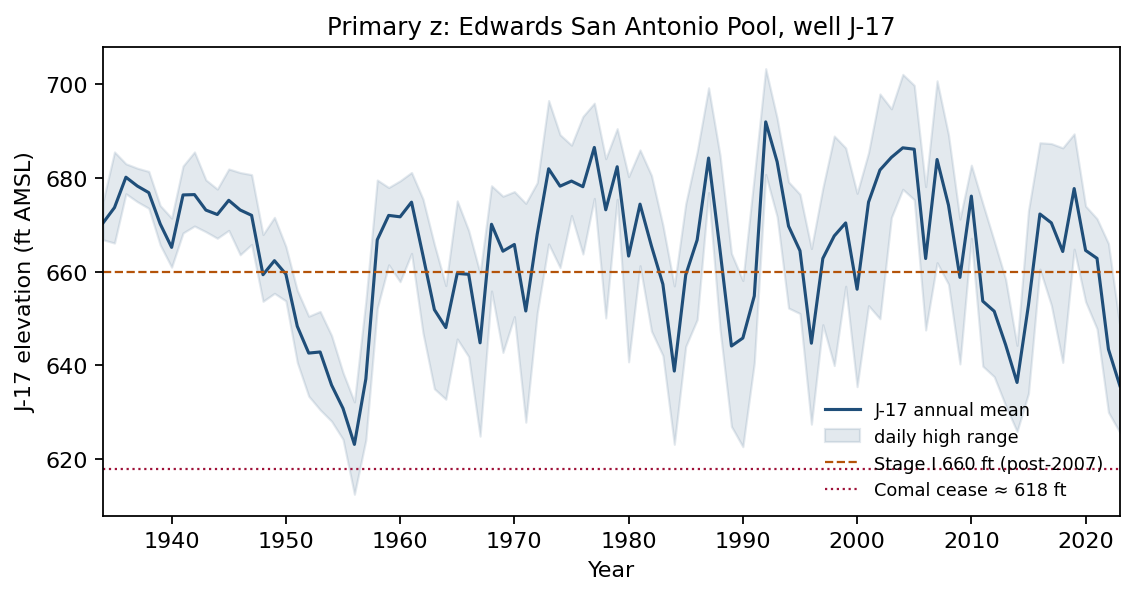
\includegraphics[width=0.92\textwidth]{edw_fig1_series}
\caption{J-17 annual mean and daily-high range, 1934--2023. 1956 mean 623.15\,ft (daily minimum 612.51\,ft); 1992 mean 691.96\,ft (daily maximum 703.31\,ft); 2023 mean 635.68\,ft. The annual mean is below the 660-ft Stage I line in 31 of 90 years.}
\label{fig:edwseries}
\end{figure}

\subsection{The water-balance ladder}\label{sec:edw_ladder}

\begin{definition}[One-pool water-balance map]\label{def:pool}
With head clipped to $[610,710]$\,ft, the one-pool map is
\begin{equation}\label{eq:pool}
H_{t+1} \;=\; \bigl[\,H_t + \alpha + \beta\tilde R_{t+1} + \gamma\tilde P_{t+1} + \delta H_t\,\bigr]_{\mathrm{clip}},
\end{equation}
where $\tilde R$ and $\tilde P$ are the flux values a forecast substitutes for the unknown year-$(t+1)$ fluxes. Forecasts are issued at the end of year $t$ from $(H,R,P)$ through $t$; $(\alpha,\beta,\gamma,\delta)$ are refitted by least squares on the training transitions at every origin.
\end{definition}

The output clip is $[610,710]$\,ft. It never binds on the observed record (annual means 623--692\,ft); it binds on the 1956-origin persisted-drought M2 path, which is emitted as 617.1, 611.6, 610, 610, 610\,ft for 1957--1961, and at the upper bound on the 1992-origin one-step M2 forecast (raw 719.1, emitted 710\,ft; SI S17). The ladder (Table~\ref{tab:edwladder}) differs from the cod ladder in one structural respect that Section~\ref{sec:synthesis} turns on: the causal rungs must \emph{substitute} something for the target-year fluxes. M2 persists last year's $(R_t,P_t)$; M2m substitutes the training-mean fluxes; M3 adds an AR(1) residual on $\Delta H$ to M2; M4 is a one-year information-delay variant kept as a symmetry control with the cod ladder (J-17 is a telemetered gauge, so the module prices a theoretical lag rather than a constraint of this system). The climate-informed variants replace persisted $R$ by a one-step forecast of $R$ from information known at $t$: an AR(1) on $R$, lagged Ni\~no~3.4, lagged climate-division precipitation, or all three; for $h>1$ the one-step recharge forecast is held constant. The realized-flux oracle receives $(R_{t+h},P_{t+h})$, which is unavailable at the origin; it is an ex-post conditional diagnostic, not a forecast and not eligible for retention. The precipitation oracle is likewise diagnostic. M1 is the univariate AR(1), $H_{t+1}=a+\varphi H_t$, scored as the output-only rung.

\begin{table}[!htb]
\centering\small
\caption{The J-17 ladder. ``Comparator'' is the next-simpler causal model under (E2); M1 has none and is tested against persistence only.}
\label{tab:edwladder}
\begin{tabularx}{\textwidth}{@{}>{\raggedright\arraybackslash}p{0.13\textwidth}>{\raggedright\arraybackslash}p{0.16\textwidth}>{\raggedright\arraybackslash}p{0.2\textwidth}L>{\raggedright\arraybackslash}p{0.14\textwidth}@{}}
\toprule
ID & Class & Fluxes substituted at $t+h$ & Role & Comparator \\
\midrule
persist & baseline & --- & $\hat H_{t+h}=H_t$ & --- \\
mean & baseline & --- & training-window mean & --- \\
M1 & autonomous AR(1) & --- & $H_{t+1}=a+\varphi H_t$ & (persistence only) \\
M2 & causal stock-flow & last $(R_t,P_t)$ persisted & candidate for retention & M1 \\
M2m & climatological stock-flow & training-mean $(\bar R,\bar P)$ & affine AR(1) by class & M1 \\
M3 & residual & as M2 & AR(1) residual on $\Delta H$ & M2 \\
M4 & delay & as M2 & information lag; symmetry control & M3 \\
M2\_Rar, M2\_Renso, M2\_Rprecip, M2\_combo & climate-informed & one-step forecast of $R$ (AR(1) on $R$; Ni\~no~3.4; precipitation; all three) & climate rung & M1 (declared) \\
M2\_oracle & diagnostic & realised target-year $(R,P)$ & ex-post conditional diagnostic; unavailable at origin & --- \\
\bottomrule
\end{tabularx}
\end{table}

\begin{remark}[Class reduction of M2m]\label{rem:class}
Under constant fluxes $\tilde R_{t+1}=\bar R$, $\tilde P_{t+1}=\bar P$, the map \eqref{eq:pool} reduces to $H_{t+1}=(1+\delta)H_t+\mathrm{const}$ and therefore shares M1's forecast function class, though not its estimator: M2m pins its intercept from the in-sample mean fluxes, an additional identifying use of the recharge and pumpage records, while the persistence coefficient $(1+\delta)$ is not mean-flux dependent. M2m passes the H1/H2 point-score gate; the separate class disposition recorded in the broader Aug.\ 27 specification sheet excludes it from the count of additional function classes. That classification is not a failure of (E1) or (E2), and it changes the structural label while leaving the score-gate result intact.
\end{remark}

\FloatBarrier
\subsection{The verdict under Protocol E, and under Protocol C}\label{sec:edw_verdict}

Table~\ref{tab:edwrolling} gives the rolling-origin summary and Fig.~\ref{fig:edwrmse} the per-model RMSE at both horizons. At $h=1$ persistence scores 13.23\,ft and the training mean 16.17\,ft. M1 scores 12.84\,ft and passes (E1); as the simplest output-only rung it has no next-simpler causal comparator, so (E2) is vacuous and M1 is retained by Protocol E's point rule. M2 (14.70), M3 (14.46) and M4 (14.30\,ft) fail (E1): the balance that persists last year's fluxes is worse than persisting the head. M2m (12.28\,ft) passes both H1/H2 inequalities against persistence and M1, then is separately declined as additional structure by the class disposition. The realized-flux diagnostic, at 7.55\,ft, is 43\% below persistence but uses unavailable target-year fluxes. Under Protocol C, restated on these scores, no module is retained: M1's 2.96\% margin is inside the 5\% band and at $h=5$ M1 (21.25\,ft) does not beat persistence (21.11\,ft). The point gate and the class disposition are reported separately because they answer different questions.

\begin{table}[!htb]
\centering\small
\caption{J-17: rolling-origin summary (ft; $n=75$ at $h=1$, $n=71$ at $h=5$, identical origin sets for every row), with Protocol E point-gate status and the separate M2m class disposition. Subscripts give the horizon; $\Delta$ columns are $h=1$ RMSE differences, negative favouring the module. The training mean is the best non-oracle forecaster at $h=5$.}
\label{tab:edwrolling}
\footnotesize\setlength{\tabcolsep}{3.5pt}
\begin{tabularx}{\textwidth}{@{}>{\raggedright\arraybackslash}p{0.19\textwidth}rrrrrL@{}}
\toprule
Model & RMSE$_1$ & MAE$_1$ & RMSE$_5$ & $\Delta$ persist & $\Delta$ M1 & Protocol E decision \\
\midrule
persist & 13.23 & 10.73 & 21.11 & --- & --- & benchmark \\
mean & 16.17 & 13.17 & \textbf{16.80} & $+2.94$ & --- & benchmark \\
M1 AR(1) & 12.84 & 10.72 & 21.25 & $-0.39$ & --- & retained (point rule; margin within noise) \\
M2 persisted fluxes & 14.70 & 11.45 & 33.49 & $+1.47$ & $+1.86$ & rejected: fails (E1) \\
M2m climatological fluxes & 12.28 & 10.22 & 17.44 & $-0.95$ & $-0.56$ & passes H1/H2; separately class-demoted \\
M3 residual & 14.46 & 11.12 & 33.46 & $+1.23$ & $+1.62$ & rejected \\
M4 delay & 14.30 & 11.17 & 33.39 & $+1.07$ & $+1.46$ & rejected \\
M2\_oracle & 7.55 & 5.79 & 10.86 & $-5.68$ & --- & excluded (uses future $R,P$) \\
\bottomrule
\end{tabularx}
\end{table}

\begin{figure}[!htb]
\centering
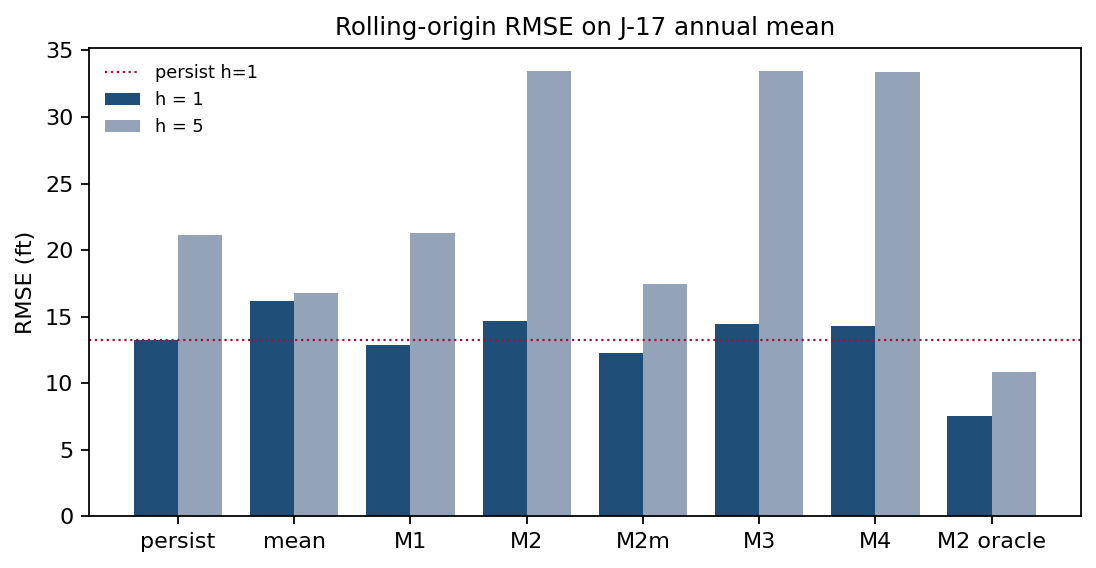
\includegraphics[width=0.8\textwidth]{edw_fig3_rmse}
\caption{J-17: rolling-origin RMSE by model at $h=1$ and $h=5$. The oracle is a diagnostic ceiling and is excluded from retention. At five years the training mean is the best non-oracle forecaster and M2--M4 are 60\% worse than persistence.}
\label{fig:edwrmse}
\end{figure}

M1's retention is a one-year point-RMSE result and should be read as such. Its 0.39\,ft margin on $n=75$ has a bootstrap interval that covers zero; MAE is a tie (10.72 versus 10.73\,ft), and the ordering reverses at five years. M2m is a second H1/H2 point-gate pass, but its affine-AR(1) class disposition is separate: without that disposition, the literal score gate would count it as retained. The score table therefore does not support the unqualified statement that no stock-flow map passes; it supports the narrower finding that persisting last year's recharge fails on these origins, while the climatological-flux affine map has the best one-step score but is not an additional forecast function class. Neither point ranking is, by itself, a claim of operational value.

\subsection{Uncertainty on the margins}\label{sec:edw_uncertainty}

Table~\ref{tab:edwdm} attaches Diebold--Mariano statistics and moving-block bootstrap intervals to the load-bearing margins, computed from the archived per-origin forecast files; the layer is post-freeze and changes no verdict. Three readings follow. The retention margin itself (M1 $-$ persist, $-0.39$\,ft) is within noise, as are the M2m-over-M1 estimator margin and the M2 causal loss (the last borderline, its interval touching zero); the only one-year margin that separates from zero is M2m over persistence ($-0.95$\,ft, $p=0.003$). The five-year climatology win ($-4.30$\,ft) is robust: its bootstrap interval excludes zero, and the $h=5$ Diebold--Mariano $p$ of 0.10 reflects the known under-sizing of that statistic under overlapping origins. And the climate-rung margins are within noise in both directions. An independent second implementation of the layer (different seed, block length $h$, 20\,000 replicates, different HAC weighting and variance convention; SI S18) reproduces every reading: M1's retention margin has $z=-0.86$ and block interval $[-1.22,+0.56]$\,ft; the M2m edge over persistence has $p=0.001$; the five-year climatology win has $p=0.035$.

\begin{table}[!htb]
\centering\small
\caption{J-17: uncertainty on the load-bearing margins (post-freeze layer; Diebold--Mariano with Newey--West HAC at lag $h-1$; paired moving-block bootstrap, block length 8, 10\,000 replicates, seeded). Rolling origin, $h=1$ unless noted.}
\label{tab:edwdm}
\scriptsize\setlength{\tabcolsep}{3pt}
\begin{tabular}{@{}lrrrcl@{}}
\toprule
Comparison & margin (ft) & DM & $p$ & 95\% block CI (ft) & separates \\
\midrule
M1 $-$ persist & $-0.39$ & $-0.85$ & 0.40 & $[-1.51,\,+0.71]$ & no \\
M2m $-$ persist & $-0.95$ & $-3.07$ & 0.003 & $[-1.45,\,-0.68]$ & \textbf{yes} \\
M2m $-$ M1 & $-0.56$ & $-1.61$ & 0.11 & $[-1.53,\,+0.13]$ & no \\
M2 $-$ persist & $+1.47$ & $+1.27$ & 0.21 & $[-0.02,\,+3.40]$ & no (borderline) \\
mean $-$ persist ($h=5$) & $-4.30$ & $-1.65$ & 0.10 & $[-9.72,\,-2.09]$ & \textbf{yes} \\
M1 $-$ persist ($h=5$) & $+0.15$ & $+0.06$ & 0.95 & $[-5.57,\,+4.94]$ & no \\
M2\_combo $-$ M1 (climate) & $-0.13$ & $-0.21$ & 0.83 & $[-1.37,\,+1.31]$ & no \\
M2\_combo $-$ M2m (nested) & $+0.43$ & $+0.74$ & 0.46 & $[-0.56,\,+1.57]$ & no \\
\bottomrule
\end{tabular}
\end{table}

\FloatBarrier
\subsection{The mechanism: a low-persistence driver, a realized-flux diagnostic, and what climate indices add}\label{sec:edw_mech}

The one-pool increment tracks same-year recharge: $r(\Delta H_t,R_t)=0.74$ on the 1934--2023 record, and the realized-flux diagnostic RMSE is 43\% below persistence at $h=1$ and 49\% below at $h=5$. The same increment is only weakly associated with last year's recharge ($r(\Delta H_t,R_{t-1})=0.06$), while recharge has a low lag-one autocorrelation ($r(R_t,R_{t-1})=0.17$, compared with 0.87 for pumpage). A module that persists $R_t$ therefore substitutes a weakly predictive value and loses to persisting head. Conditioned on the realised target-year fluxes, the same map scores 7.55\,ft; this ex-post conditional diagnostic uses information unavailable at the origin and is not an origin-available forecast. It shows that the fitted map can track the realised increment when supplied its drivers; it does not establish operational skill for predicting the next increment.

The fixed windows make the point visibly (SI S17). The 1957--1961 recovery from the drought of record is a recharge pulse ($R_{1956}=43.7$, $R_{1957}=1142.6\times10^3$ acre-ft): persistence stays at the 1956 floor (RMSE 43.6\,ft), M2 persists drought recharge and falls further, into the clip (55.3\,ft), and the oracle tracks the rise (12.3\,ft). The 1992 peak and the 2015--2023 window repeat the split. On the 1951--1956 drawdown M2 ``beats'' the oracle (18.1 against 19.7\,ft), but for a reason that undermines it: the map trained on 1934--1950 has the wrong sign on pumpage ($\gamma=+0.021$), because pumping rose as the drought deepened and least squares aliases the human response into the state transition.

The climate-informed variants ask whether signals observable at the annual origin (September--November Ni\~no~3.4, lagged climate-division precipitation, and an AR(1) on $R$) supply a useful recharge forecast (Table~\ref{tab:edwclimate}). On the recharge target, the climate modules score 528--545 against the $556\times10^3$ acre-ft climatology; persisted recharge scores 702. Under the pre-score Pass~2 H1/H2 point gate, which compares against persistence and M1, Renso, Rprecip and combo pass at $h=1$; Rar fails. These point-gate outcomes are distinct from the archived class assessment, which demotes the three passes as M2m-plus-intercept variants rather than additional head-forecast structure, leaving \texttt{retained\_as\_structure} empty. Against M2m as an alternative comparator none clears the strict point gate; this alters the point-gate count but not the separate class result. The edges over M1 are only 0.02--0.13\,ft; the reported combined-rung uncertainty interval covers zero (Table~\ref{tab:edwdm}). All four climate variants are 3--6\,ft worse than persistence at $h=5$, in part because the one-step recharge forecast is held constant over the horizon. The Pass~2 score outcomes are reported as written, while the uncertainty and longer-horizon results qualify interpretation rather than retroactively changing the gate. Fixed-window results, including the one window on which two variants edge M1 by about a foot, are in SI S22. Same-year precipitation, unavailable at the origin, yields 10.56\,ft as a conditional diagnostic; it remains above the realized-flux diagnostic because the linear rain map misses 1957-scale extremes. Neither diagnostic forecasts next year's recharge.

\begin{table}[!htb]
\centering\scriptsize\setlength{\tabcolsep}{2pt}
\caption{J-17: climate-informed recharge, rolling origin on the same sets as Table~\ref{tab:edwrolling}. Head RMSE in ft; recharge RMSE in $10^3$ acre-ft. The final column separates point-gate status from the archived structural-class disposition; neither is an uncertainty test. Renso, Rprecip and combo pass the Pass~2 point gate but are class-demoted; M2m's separate Pass~1 result is shown for comparison.}
\label{tab:edwclimate}
\begin{tabularx}{\textwidth}{@{}>{\raggedright\arraybackslash}p{0.20\textwidth}rrrr>{\raggedright\arraybackslash}X@{}}
\toprule
Model & $H$, $h{=}1$ & margin vs.\ M1 & $H$, $h{=}5$ & $R$, $h{=}1$ & Point gate / class status \\
\midrule
persist $H$ / persist $R$ & 13.23 & $+0.39$ & \textbf{21.11} & 702 & benchmark \\
M1 & 12.84 & --- & 21.25 & --- & Pass~1 retained rung; Pass~2 comparator \\
M2\_Rar & 13.25 & $+0.41$ & 25.38 & 561 & fails Pass~2 H1/H2 \\
M2\_Renso & 12.82 & $-0.02$ & 24.42 & 528 & passes Pass~2; class-demoted \\
M2\_Rprecip & 12.80 & $-0.04$ & 25.38 & 545 & passes Pass~2; class-demoted \\
M2\_combo & 12.71 & $-0.13$ & 26.88 & 538 & passes Pass~2; class-demoted \\
M2m climatological fluxes & 12.28 & $-0.56$ & 17.44 & --- & passes Pass~1; separately class-demoted \\
recharge climatology & --- & --- & --- & 556 & benchmark \\
precipitation oracle (year $t{+}h$) & 10.56 & --- & 16.91 & \textbf{354} & conditional diagnostic; future input \\
\bottomrule
\end{tabularx}
\end{table}

\subsection{Post-freeze layers: the service series and the pumpage counterfactuals}\label{sec:edw_post}

Two layers were scored after retention was frozen and change no verdict; both are reported in full in the SI. The Comal Springs discharge series is a near-linear channel of the same state ($r=0.986$ with J-17): rescoring the ladder on the same origins gives a broadly similar ordering (persist 71.9, M1 69.0, M2m 68.7, M2 74.8\,cfs; realized-flux diagnostic 45.3), as expected from a near-linear channel but not mathematically guaranteed. The channel is least redundant with head in the drought tail, where the fitted rating curve predicts about 97\,cfs at the 1956 mean against an observed 32 and fails to signal cessation (SI S20). The pumpage counterfactuals replay actual recharge through the short pre-permit map from the 1990 head; they are illustrative simulations, not forecasts or policy estimates. Across the four paths, the 2023 head spans 630.9--646.8\,ft, comparable to the map's 7.2--14.2\,ft RMSE against observations. This makes pumpage a secondary lever within this fitted map; the coefficient is subject to the drawdown-window simultaneity caveat and no scenario repairs the ladder's primary failure (SI S21).

\subsection{Reading the aquifer verdict}\label{sec:edwreading}

Three statements survive the uncertainty layer. First, the causal balance that persists last year's recharge is not a one-year forecast winner on this origin set; the evidence points to low recharge persistence rather than an inability of the map to track a realised transition. The 7.55\,ft realized-flux score is conditional on target-year drivers, so it does not measure prospective forecast skill. Second, M1's Protocol E retention is a weak-autocorrelation result, not evidence that output-only models are generally preferable. An estimated AR(1) nests persistence at $\varphi=1$; as the head series approaches that limit the forecasts converge and the AR(1)'s advantage shrinks toward estimation noise. Here the head is persistent but far from a unit root (lag-one autocorrelation 0.63; fitted $\hat\varphi=0.66$), leaving a real but slim point margin.  The fitted $\hat\varphi=0.66$ also has a physical reading: under first-order Darcy proportionality, spring discharge above the spring level implies an affine autonomous form $H_{t+1}\approx(1-k)H_t+kH_s$, with $\hat k\approx0.34$\,yr$^{-1}$. Third, on these rolling origins the training mean beats persistence at five years (16.80 versus 21.11\,ft; bootstrap interval excludes zero). This is a benchmark-specific result for a rapidly recharged, institutionally bounded aquifer, not a general multi-year rule; it need not transfer to a non-stationary fossil aquifer under sustained depletion. Section~\ref{sec:synthesis} states the narrower conditions under which a mean-reverting baseline is informative.
\FloatBarrier
\section{Cross-system synthesis: contrasting forecast deficits, one decomposition}\label{sec:synthesis}

The two systems were scored separately and will stay separate; what they share is a question and, it turns out, an arithmetic. Both ladders consist of \emph{increment forecasters}: each module forecasts next year's state as this year's state plus a mechanism, and the mechanism is evaluated at whatever the module can substitute for the quantities it needs but does not know. On cod the stock-flow modules receive catch while the autonomous modules substitute its training mean and retain state-dependent production; on J-17 M2 substitutes last year's recharge, M2m its climatological mean and the conditional diagnostic the realized value. Persistence is the increment forecaster with mechanism zero. The following proposition says exactly how such a forecaster can gain or lose against it.

\subsection{The increment decomposition}\label{sec:decomp}

\begin{proposition}[One-step skill of an increment forecaster]\label{prop:increment}
Let $\Delta_{t+1}=y_{t+1}-y_t$ and let a forecaster issue $\hat y_{t+1}=y_t+m(\hat x_{t+1})$, where $m$ is its mechanism, $x_{t+1}$ the driver at which the mechanism would be evaluated if the driver were known, and $\hat x_{t+1}$ the value substituted at the origin. Write $m_{t+1}=m(x_{t+1})$, $u_{t+1}=\Delta_{t+1}-m_{t+1}$ (the mechanism residual) and $d_{t+1}=m_{t+1}-m(\hat x_{t+1})$ (the substitution error). Then, whenever the second moments exist,
\begin{equation}\label{eq:decomp}
\MSE(\hat y)-\MSE(\pers)\;=\;\underbrace{\E[d_{t+1}^2]-\E[m_{t+1}^2]}_{\text{substitution term}}\;-\;\underbrace{2\,\E\bigl[u_{t+1}\,m(\hat x_{t+1})\bigr]}_{\text{misspecification term}} .
\end{equation}
In particular:
\begin{enumerate}[label=(\roman*),leftmargin=2.2em,itemsep=2pt]
\item \emph{Supplied driver.} If $\hat x_{t+1}=x_{t+1}$ then $d\equiv0$ and $\MSE(\hat y)-\MSE(\pers)=\E[u_{t+1}^2]-\E[\Delta_{t+1}^2]$: the forecaster beats persistence if and only if its mechanism residual is smaller in mean square than the increment itself.
\item \emph{Persisted driver.} If $\hat x_{t+1}=x_t$, the sequence $m_t$ is weakly stationary with mean $\mu$, variance $\sigma^2$ and lag-one autocorrelation $\rho$, and $\E[u_{t+1}m_t]=0$, then
\[\MSE(\hat y)-\MSE(\pers)\;=\;\sigma^2(1-2\rho)-\mu^2,\]
so the forecaster beats persistence if and only if $\rho>\tfrac12-\mu^2/(2\sigma^2)$. For a mean-zero mechanism this is $\rho>\tfrac12$, whatever the mechanism's fidelity.
\item \emph{Constant substituted mechanism.} If the entire forecast increment satisfies $m(\hat x_{t+1})=\mu$ and $\E[u_{t+1}]=0$, then $\MSE(\hat y)-\MSE(\pers)=-\mu^2\le0$: this constant-increment forecaster never loses to persistence, and it beats the persisted-driver forecaster of (ii) by $\sigma^2(1-2\rho)$, which is positive if and only if $\rho<\tfrac12$. A model with climatological flux inputs but a head-dependent drain does not, in general, satisfy this condition.
\end{enumerate}
\end{proposition}

The proof is in \ref{app:proofs}. The identity is exact; its special-case readings require their stated assumptions. When a driver is persisted, the half-autocorrelation threshold follows only for a weakly stationary, mean-zero mechanism with zero residual cross-term. The $-\mu^2$ result applies only when the \emph{entire} substituted increment is constant, not merely when one set of inputs is replaced by its training mean. In general, the substitution term depends on the difference between the realized and substituted mechanisms, while the residual cross-term depends on how the mechanism error co-moves with the forecast actually issued. A structural forecaster can therefore lose to persistence through a substitution penalty partly offset or amplified by residual covariance. Cod supplies the driver at one step, making the misspecification comparison direct; the J-17 rolling application below reports both terms rather than imposing the stationary special case.

\paragraph{J-17: substitution penalty and residual covariance.} For each one-step rolling origin, let $m_{t+1}$ be the fitted M2 increment evaluated at the realized target-year $(R_{t+1},P_{t+1})$ and origin-known $H_t$, and let $\hat m_{t+1}$ use the persisted $(R_t,P_t)$ with the same fitted coefficients and $H_t$. The general identity, evaluated before clipping and with all 75 origin-specific fits, gives an empirical substitution contribution $\overline{d^2-m^2}=+76.03$\,ft$^2$ and residual cross-term $-2\overline{u\hat m}=-27.49$\,ft$^2$, for a raw M2-minus-persistence gap of $+48.54$\,ft$^2$ (SI S23). The $[610,710]$ output clip binds once in this one-step rolling set, at the 1992 origin; the scored gap is $14.70^2-13.23^2=+40.99$\,ft$^2$. Thus driver substitution is the larger adverse term, but it is not the whole forecast-error difference. The full-sample flux component $\hat\beta R_t+\hat\gamma P_t$ has lag-one autocorrelation about 0.08 (standard deviation 9.2\,ft); recharge itself has autocorrelation 0.17, and $r(\Delta H_t,R_t)=0.74$ versus $r(\Delta H_t,R_{t-1})=0.06$. These diagnostics support a low-persistence driver interpretation, but the half-autocorrelation special case is not an exact numerical prediction for this fitted model: its increment also contains the state-dependent drain, and the residual cross-term is nonzero. M2m's 12.28\,ft RMSE is an observed point-score pass; because its affine increment retains the head-dependent drain, it does not instantiate the theorem's constant-increment corollary. The realized-flux score of 7.55\,ft is a conditional diagnostic using future fluxes, not forecast skill. Fig.~\ref{fig:mechanism}a--b shows the separate driver and increment correlations.

\paragraph{Cod fails on the misspecification term.} The stock-flow modules are case (i): the catch is supplied, $d\equiv0$, and their deficit is entirely $\E[u^2]-\E[\Delta^2]$, the mechanism residual against the raw increment. Proposition~\ref{prop:repeller}(ii) says what that residual is in the collapse years: the realised increments $\Delta_{t+1}=S_{t+1}-S_t$ lay 66--161\,kt (coarse regime) and 59--240\,kt (annual landings) below $-C_t$, so $u=\Delta_{t+1}+C_t-g(S_t)<0$ for every nonnegative production curve, and $|u|>|\Delta_{t+1}|$ exactly when $g(S_t)>C_t$, that is, whenever the fitted production exceeds the supplied catch, which is the situation of a module told that removals are falling. The autonomous modules replace catch with its training mean, but their production term remains state-dependent; neither the persisted-driver special case nor the constant-increment corollary applies. After 1992 that substituted catch greatly exceeds production at the depleted stock, the map is driven to the floor, and the residual equals the observed biomass at every origin. Neither failure has anything to do with the predictability of a driver: the apparent net production of the assessed series is strongly autocorrelated (lag-one autocorrelation 0.75 on Specification A under the coarse regime, 0.71 under annual landings, 0.91 on Specification B), and the attribution of the cod result to a ``weakly autocorrelated surplus production'' in an earlier combination of these studies is withdrawn. The cod modules fail because the class cannot represent the transitions that carry the error; the simulations show high sensitivity for the D1 collapse-fit autonomous truth, but low power for the tested stock-flow truth, so non-retention of the catch-supplied modules does not rule out that structure.

\subsection{When climatology overtakes persistence}\label{sec:crossover}

The same arithmetic settles the relation between the two baselines, which the five-year J-17 result raised.

\begin{remark}[Horizon crossover of the baselines]\label{rem:crossover}
If $y$ is weakly stationary with variance $\sigma_y^2$ and lag-$h$ autocorrelation $\rho_h$, and the climatological mean is known, then $\MSE_h(\pers)=2\sigma_y^2(1-\rho_h)$ and $\MSE_h(\mathrm{mean})=\sigma_y^2$, so $\RMSE_h(\pers)/\RMSE_h(\mathrm{mean})=\sqrt{2(1-\rho_h)}$ and the training mean overtakes persistence at the first horizon at which $\rho_h<\tfrac12$. With an estimated mean the ratio is shifted by the estimation variance of the mean, which is small relative to $\sigma_y^2$ for long training windows.
\end{remark}

Fig.~\ref{fig:mechanism}c tests the remark on all three series with the baselines recomputed at every horizon $h=1,\dots,5$ on the registered data and on the origin sets of the scored ladders (the $h=1$ and $h=5$ values reproduce Tables~\ref{tab:rolling} and \ref{tab:edwrolling} exactly; SI S23). On J-17 the head's autocorrelation falls from 0.63 at lag one to 0.35 at lag two, so the remark predicts that climatology overtakes persistence between one and two years; the observed ratios are 0.82, 1.07, 1.22, 1.27 and 1.26 against predicted 0.86, 1.14, 1.31, 1.37 and 1.36, the crossover is at $h=2$, and the five-year result of Section~\ref{sec:edwards} is the plateau of that curve rather than an isolated finding. On cod the SSB series is not stationary over the scored windows (a collapse by an order of magnitude and a partial rebuild), the training mean of a collapsing series is a poor estimate of anything, and the remark fails in the direction it should: the observed ratios stay between 0.18 and 0.58 at every horizon while the stationary formula would predict a crossover between four and five years on Specification A. The criterion is therefore a test as well as a prediction. A close match between $\sqrt{2(1-\hat\rho_h)}$ and the observed baseline ratio indicates that the stationary identity approximates the scored comparison on that series; a mismatch indicates that its assumptions do not describe the series. Neither reading is a policy rule, and neither transfers without a system-specific evaluation.

\begin{figure}[!htb]
\centering
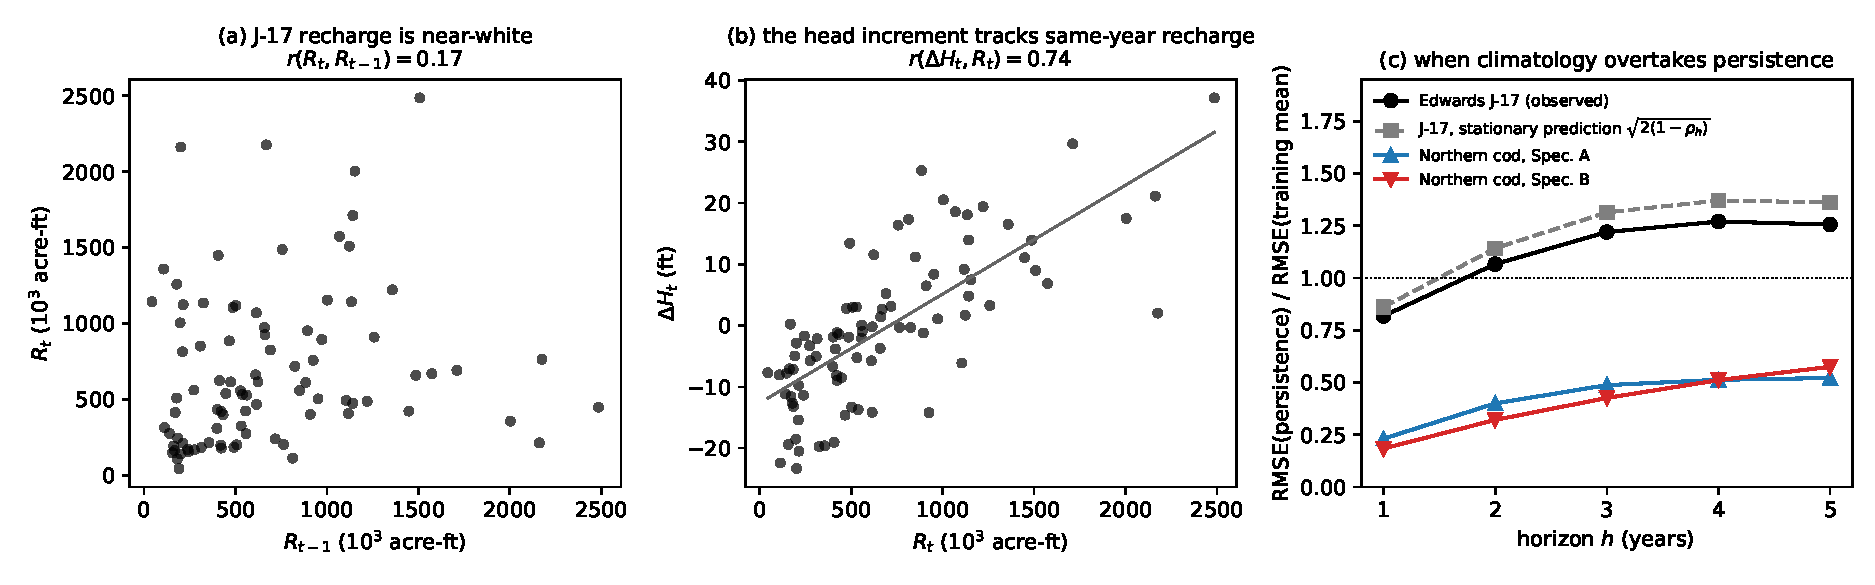
\includegraphics[width=\textwidth]{fig7_mechanism}
\caption{Driver, increment and baseline diagnostics. (a) J-17 annual recharge is weakly persistent: $R_t$ against $R_{t-1}$, $r=0.17$. (b) The J-17 head increment is associated with same-year recharge: $\Delta H_t$ against $R_t$, $r=0.74$; the realized-flux score is conditional on future drivers, and the exact rolling M2 decomposition retains both the substitution and residual-cross terms (SI S23). (c) Ratio of rolling-origin persistence RMSE to training-mean RMSE by horizon on the scored origin sets: J-17 observed (black) against the stationary prediction $\sqrt{2(1-\rho_h)}$ of Remark~\ref{rem:crossover} (grey, dashed), with the crossover at $h=2$; Northern cod Specifications A and B never cross within five years, and the stationary prediction does not apply to them.}
\label{fig:mechanism}
\end{figure}

\subsection{What transfers and what does not}\label{sec:transfer}

Table~\ref{tab:cross} sets the two systems side by side without pooling them. What transfers is an analytic distinction: compare each forecast with origin-matched simple baselines at declared horizons, state the information set and the model-class rule, and keep the exact decomposition's substitution and residual terms separate. On J-17, the realized-flux diagnostic shows how the fitted map scores when supplied target-year drivers, but it is not an operational forecast; the annual-origin climate variants do not recover the recharge pulse in the drought-recovery window. Any within-year data-update forecast would require its own origin definition and evaluation, and no such result is claimed here. On cod, the catch-supplied modules carry a short-memory growth component with one-step skill in a low-biomass band on one specification; this is a hypothesis for a future test with an externally fixed regime boundary and consistent catch timing, not a management recommendation. What does not transfer is any score, margin, autocorrelation or operating characteristic: those results belong to the tested series and information sets, and another system requires its own evaluation.

\begin{table}[!htb]
\centering\small
\caption{The two systems side by side. Nothing in this table is pooled; each column is one series under its own protocol. ``Failing term'' refers to equation~\eqref{eq:decomp}.}
\label{tab:cross}
\begin{tabularx}{\textwidth}{@{}>{\raggedright\arraybackslash}p{0.21\textwidth}LL@{}}
\toprule
 & Northern cod (Spec.\ A; Spec.\ B) & Edwards J-17 \\
\midrule
Predictand & assessed SSB, kt; retrospective vintage & measured annual-mean head, ft \\
Structural claim & surplus production; catch-driven stock flow; depensation; residual memory & one-pool water balance; residual and delay variants; climate-informed recharge \\
Driver at the origin & catch supplied (M2--M4) or held at training mean (M1, M1b) & recharge and pumpage persisted (M2), climatological (M2m), forecast from climate indices, or realised (oracle) \\
Protocol & C: 5\% band, both horizons, comparator and persistence & Pass~1 H1/H2 at $h=1$; separate M2m class disposition; Pass~2 H1/H2 against persistence and M1 \\
One-year persistence RMSE & 98.0; 84.4\,kt & 13.23\,ft \\
Best point-score module at $h=1$ & M1b 114.8 (ratio 1.17); M1 119.5 (1.42) & M2m 12.28 (H1/H2 pass, class-demoted); M1 12.84 (retained) \\
Structural disposition & none; none & Pass~1: M1 retained, M2m class-demoted; Pass~2: three point-gate passes class-demoted; none under C \\
Error decomposition & misspecification: collapse transitions outside the class; floor forecasts after 1992 & M2 substitution term $+76.0$\,ft$^2$, residual cross-term $-27.5$\,ft$^2$; clipped MSE gap $+41.0$\,ft$^2$ \\
Lag-one autocorrelation & apparent net production 0.75; 0.91 & flux component 0.08; recharge 0.17 \\
Baseline crossover (Remark~\ref{rem:crossover}) & none within five years; stationary formula inapplicable & at $h=2$, as predicted on these origins \\
Operating-characteristic evidence & D1 true-M1 power 95.0--97.5\%; D3 true-M2 power 10.5--13.0\%; D5 any-module false retention 2.5--7.5\% (point specificity 92.5--97.5\%) & 7.55\,ft realized-flux conditional diagnostic, not power; climate point margins $\le0.13$\,ft \\
\bottomrule
\end{tabularx}
\end{table}
\FloatBarrier
\section{Related work and what is new}\label{sec:related}

\paragraph{Forecast evaluation.} Comparing the out-of-sample accuracy of competing forecasters on the same realisations, rather than their in-sample fit, is the established discipline for the question asked here \citep{Diebold1995,HyndmanKoehler2006,HyndmanAthanasopoulos2021}, and rolling-origin evaluation is its standard form for time series \citep{Tashman2000,Bergmeir2012}. The hazard that discipline guards against is selection after the fact: when many candidates are scored on one realisation, the best observed score is an upward-biased estimate of skill and per-comparison tests do not restore validity. White's reality check constructs the distribution of the best statistic across candidates under the null that none has skill \citep{White2000}, and stepwise procedures formalise the correction with control of the familywise error rate \citep{RomanoWolf2005}. The present design addresses the same hazard by a more restrictive and less general route, and the difference should be stated. Those procedures take a set of already-computed scores and ask which survive correction for having been selected. Here the model classes, baselines and scoring cores were declared for each system; the Edwards H1/H2 gates were frozen before their respective scores, while the cod 5\% band and some comparator declarations were formalised after the first pass. These completions are disclosed, and the operating characteristics are estimated by simulation conditional on the cod rule as applied. This design is not a familywise-error correction and is not presented as one.

\paragraph{Simple benchmarks are hard to beat.} That naive and simple statistical methods are close to the most accurate, and that sophisticated methods frequently fail to beat them, is the most consistently replicated result in forecasting: it organises the M3 and M4 competitions \citep{Makridakis2000,Makridakis2018}, in the latter of which none of the pure machine-learning entries was more accurate than the combination benchmark, and it has been found on fish population series \citep{Ward2014} and on simulated ecological dynamics \citep{Perretti2013}. The two results here are single-system instances of that phenomenon, and the scope difference is material: the competitions aggregate over tens of thousands of series and dozens of methods, whereas this paper scores two ladders on two systems. A cross-series result about method classes entails nothing about a particular stock or basin, and a two-system result does not generalise to method classes. What the two kinds of result share is the test, and what this paper adds to the phenomenon is a reason, in equation~\eqref{eq:decomp}, why a mechanistic increment forecaster loses to persistence when it does.

\paragraph{Fisheries.} Structural claims in stock assessment are usually examined through fit, retrospective pattern and simulation self-consistency \citep{HilbornWalters1992,Punt2016,Maunder2015}; where prediction skill is examined directly, it is computed on the fitted survey or catch-rate index through hindcast cross-validation \citep{Kell2016,Kell2021,Carvalho2021,Kokkalis2024}, while advice concerns the state, and the difficulties of fitting surplus-production models to series with little contrast are long documented \citep{HilbornWalters1992,LudwigWalters1985,Polacheck1993,Punt2003,PedersenBerg2017}. The Northern cod collapse and its non-recovery have an extensive literature establishing the empirical facts \citep{Hutchings1994,Myers1997,Walters1996,Hutchings2005,RoseRowe2015,RoseWalters2019,Rose2026} and debating depensation \citep{Shelton1999,Hutchings1996,Myers1995,Liermann1997}. This paper's contribution to that literature is different in kind: it measures what those facts do to the forecast skill of a familiar model class from fixed origins, locates the deficit in the collapse transitions, proves that those transitions lie outside the class at the recorded catch, and reports the power of the test. It is a conditional hindcast, scored against a retrospective vintage with catch supplied along the horizon; it is not an operational forecast evaluation and licenses no claim about the performance of the assessment process as it ran.

\paragraph{Groundwater.} Groundwater-level forecasting at index wells is a mature area with statistical, neural-network and process-based approaches on annual and sub-annual series \citep{Daliakopoulos2005,AdamowskiChan2011}, and it has begun to institutionalise benchmark culture: GEMS-GER standardises 32 years of weekly observations from 3\,207 German wells with three benchmark models of increasing complexity \citep{Ohmer2026}, and a systematic comparison of nine machine-learning architectures on a karst catchment finds that aquifer complexity rather than algorithm choice bounds predictability \citep{Zhu2026}. Those studies compare model families against one another. None subjects a deliberately simple process-based water balance to a scored ablation against persistence and the training mean under a dated pre-score computational gate, and none reports a training mean beating persistence at a multi-year horizon on this basin. On the Edwards Aquifer, regional flow has long been represented, and debated, through equivalent-porous-media and lumped approaches \citep{Scanlon2003}; the one-pool map is not a karst model and the lumped-versus-distributed question is inherited rather than settled here. The climate predictors enter because ENSO phases shift North American precipitation \citep{Ropelewski1986}, and the finding that they add at most 0.13\,ft at the annual origin is a statement about this information set, not about ENSO.

\paragraph{What is new.} Relative to the two single-system studies and their earlier two-part combination, this article contributes (a) one scored test reported on two systems under disclosed, system-specific point rules without pooling, with the Edwards score gates and class dispositions separated; (b) Proposition~\ref{prop:increment}, an exact one-step MSE identity separating driver substitution from residual covariance, with a half-autocorrelation threshold only under the stated stationary, mean-zero and orthogonality conditions, and a constant-increment corollary; (c) Remark~\ref{rem:crossover}, the half-autocorrelation crossover of persistence and the training mean, evaluated on J-17 origins and shown not to describe the non-stationary cod series; (d) the correction of the earlier cross-system reading, which attributed the cod failure to a weakly autocorrelated driver; and (e) for the cod half, the period decomposition, identification result and operating characteristics, reported alongside—but not equated with—the J-17 realized-flux conditional diagnostic, which uses unavailable future drivers and is not an operating-characteristic estimate.
\FloatBarrier
\section{Discussion}\label{sec:discussion}

\subsection{Why a negative result is informative here}\label{sec:whyinformative}

A negative result is interpretable only relative to the rule, the sensitivity of the test and the location of the error. The chronology is qualified rather than prospective: the Edwards H1/H2 gates were frozen and archived before their respective score passes, while the cod 5\% band and some comparator declarations were formalised after its first pass; none of the disclosed completions changes the cod verdict. Cod operating characteristics are estimated by simulation under the specified data-generating processes. J-17 has a different, non-equivalent diagnostic: the realized-flux score of 7.55\,ft conditions on target-year drivers unavailable at the origin and is neither a power estimate nor forecast-skill evidence. Proposition~\ref{prop:increment} gives an exact identity, and the rolling J-17 application shows a $+76.0$\,ft$^2$ substitution term partly offset by a $-27.5$\,ft$^2$ residual cross-term before clipping; the one-step output cap reduces the observed M2--persistence gap to $+41.0$\,ft$^2$ (SI S23). On cod, the deficit is a misspecification term concentrated in the 1991--1995 transitions, which no member of the tested class can produce at the recorded catch (Proposition~\ref{prop:repeller}). On J-17, the low persistence of the flux component helps explain why carrying last year's recharge performs poorly, but the exact score gap is not attributable to substitution alone. Any forecast using partial-year recharge would need a separately defined origin and evaluation; it is not evaluated here. A future cod test of the low-biomass pattern would likewise need an external regime boundary, consistent catch timing, and the declared score rule applied to both series.

\subsection{Protocols, bands and the AR(1)}\label{sec:protocoldiff}

The cod and Edwards point rules disagree about M1: its 0.39\,ft one-year margin passes the Edwards H1/H2 gate but not the cod 5\% two-horizon gate, because 2.96\% lies inside the band and the five-year ordering reverses. The Edwards bootstrap interval covers zero in both implementations and MAE is a tie, so the point-rule retention is weak evidence of material gain; we nevertheless report it as the frozen H1/H2 rule dictates, not as a general advantage of output-only models. The class decisions are a separate issue. M2m passes Pass~1 H1/H2 and is excluded from the count of additional function classes by the broader frozen specification; its $-0.95$\,ft margin over persistence is the only one-year benchmark margin that separates from noise. In Pass~2, Renso, Rprecip and combo pass the point gate against persistence and M1, but the archived class assessment demotes them as M2m-plus-intercept variants; Rar fails the point gate. Thus the empty Pass~2 structure set is a class outcome, not a score-gate failure. Reporting the score and the class decision separately preserves both the numerical result and the protocol's declared structural interpretation.

\subsection{Limitations}\label{sec:limits}

The test covers two systems, three series, two model classes and two horizons; it is a demonstration and a replication, not a survey. On cod, each specification uses a single retrospective vintage, which favours the models (the 1983--2015 overlap between vintages differs by 24.7\,kt on average and by 131\,kt in one year); catch enters as a point series although both assessments treat it as bounded and the collapse years are under-reported; forecasts are point forecasts scored by RMSE and MAE rather than predictive distributions; Specification A has few origins; period bands were chosen after seeing the data; the archived runner's catch-timing offset moves catch-supplied one-step margins by 20--75\,kt without moving the verdict; and the operating-characteristic results cover only the declared in-class truths and two specific out-of-class truths. On J-17, recharge and pumpage are total-area estimates that mix the San Antonio and Uvalde pools, recharge is estimated by the stream-loss method, pumpage includes unreported use and is partly an institutional response to head, the map is not a karst model, the sample has four short fixed windows, and the nClimDiv precipitation source file is not redistributed (its provenance is recorded, and the scored panel is archived). The identity in Proposition~\ref{prop:increment} is exact, but the half-autocorrelation shortcut additionally requires stationarity, a mean-zero mechanism and a zero residual cross-term. The J-17 application therefore uses the full origin-specific increment and reports both empirical terms; the realized-flux diagnostic conditions on future inputs, and the output clip changes the scored error gap. Remark~\ref{rem:crossover} is a separate stationary benchmark identity; its approximation on J-17 does not establish stationarity, and it does not describe the cod series. Neither system used a prospective registration, and no such status is claimed.

\section{Conclusions}\label{sec:conclusions}

Across two unrelated systems, process-based forecast ladders were evaluated against persistence and the training mean under distinct, system-specific protocols. No surplus-production module was retained on either Northern cod assessment series; the principal failures coincide with the 1991--1995 collapse, which the tested model class cannot generate at the recorded catch. On J-17, M2's persisted-flux forecast has 14.70\,ft RMSE versus 13.23\,ft for persistence. The one-year M2m and Pass~2 climate variants pass their point gates, but the broader frozen specification classifies them as variants of the same affine-AR(1) function class; the separate Pass~1 M1 point-rule retention has a margin within uncertainty. No additional Edwards structure is retained by the class screen. The exact rolling-origin identity makes the J-17 score comparison more precise: driver substitution contributes $+76.03$\,ft$^2$, residual covariance contributes $-27.49$\,ft$^2$, and the raw MSE gap is $+48.54$\,ft$^2$; the single upper output clip reduces the archived scored gap to $+40.99$\,ft$^2$. A 7.55-ft realized-flux result is conditional on future inputs and is not forecast skill. The half-autocorrelation threshold is a special case of the identity, not a substitute for its full terms; the separate stationary baseline comparison crosses at $h=2$ on the J-17 origins and does not describe cod. These results distinguish process fidelity, information available at forecast origin, point-score evidence and structural-class evidence. They support no general claim about other systems: each inference is bounded by the series, origins and model classes evaluated here.
\appendix
\FloatBarrier
\section{Proofs}\label{app:proofs}

\paragraph{Proof of Proposition~\ref{prop:repeller}.} Throughout, $F_C(S) = \max(S + g(S) - C,\,0)$; the numerical floor $\epsilon = 10^{-3}\kt$ used in the computations replaces $0$ by $\epsilon$ and changes nothing below.

\emph{(i)} Let $0 \le S < S_-(C)$. If $g(S) \ge C$ then $S$ belongs to the set $\{S'>0 : g(S')\ge C\}$ (for $S>0$) or $g(0)=0\ge C>0$ (for $S=0$), both impossible; hence $g(S) < C$ and $S + g(S) - C < S$. Therefore $0 \le F_C(S) \le \max(S,0) = S < S_-(C)$. By induction a trajectory started in $[0,S_-(C))$ is nonincreasing and never leaves the interval. If $g(S) \ge C$ on an interval $I$ and $S\in I$, then $S + g(S) - C \ge S \ge 0$, so $F_C(S) = S + g(S) - C \ge S$.

\emph{(ii)} Suppose $S_{t+1} = F_{C_t}(S_t) < S_t - C_t$. If the maximum in $F_{C_t}$ is attained by the first argument, $S_t + g(S_t) - C_t < S_t - C_t$ gives $g(S_t) < 0$. If it is attained by $0$, then $S_t + g(S_t) - C_t \le 0 < S_t - C_t$ (the right inequality because $S_{t+1} = 0 < S_t - C_t$), and again $g(S_t) < 0$. On the compensatory branch $g(S) = rS(1-S/K) \ge 0$ for $0 \le S \le K$. On the depensatory branch $g(S) = rS(1-S/K)(S-\sA)/(K-\sA)$ with $0<\sA<K$, which for $0<S<K$ is negative exactly when $S<\sA$. \qed

For the Schaefer branch the equation $g(S)=C$ has the roots $S_\pm(C) = \tfrac{K}{2}\bigl(1\pm\sqrt{1-4C/(rK)}\bigr)$ when $4C\le rK$, $g\ge C$ on $[S_-,S_+]$ and $g<C$ outside, so $S_-(C)$ in the proposition is the lower root and $[S_-(C),S_+(C)]$ the interval on which the autonomous map cannot decline. $F_C'(S_+) = 1 + g'(S_+) = 1 + r(1-2S_+/K)$, which at the collapse-window fit under $C=240\kt$ equals $-0.39$.

\paragraph{Proof of Proposition~\ref{prop:increment}.} The forecast error of $\hat y$ is $\Delta_{t+1}-m(\hat x_{t+1}) = (m_{t+1}-m(\hat x_{t+1})) + (\Delta_{t+1}-m_{t+1}) = d_{t+1}+u_{t+1}$, and the error of persistence is $\Delta_{t+1} = m_{t+1}+u_{t+1}$. Hence
\begin{align*}
\MSE(\hat y)-\MSE(\pers) &= \E[d^2]+2\E[du]+\E[u^2] - \E[m^2]-2\E[mu]-\E[u^2]\\
&= \E[d^2]-\E[m^2] + 2\E\bigl[u\,(d-m_{t+1})\bigr],
\end{align*}
and $d-m_{t+1} = -m(\hat x_{t+1})$, which is \eqref{eq:decomp}.

\emph{(i)} With $\hat x_{t+1}=x_{t+1}$, $d\equiv 0$ and \eqref{eq:decomp} reads $-\E[m^2]-2\E[um] = \E[u^2]-\E[(u+m)^2] = \E[u^2]-\E[\Delta^2]$.

\emph{(ii)} With $\hat x_{t+1}=x_t$, $d_{t+1}=m_{t+1}-m_t$, and weak stationarity gives $\E[d^2] = 2\sigma^2 - 2\operatorname{cov}(m_{t+1},m_t) = 2\sigma^2(1-\rho)$ and $\E[m^2]=\sigma^2+\mu^2$. The misspecification term is $-2\E[u_{t+1}m_t]=0$ by hypothesis. Hence $\MSE(\hat y)-\MSE(\pers) = 2\sigma^2(1-\rho)-\sigma^2-\mu^2 = \sigma^2(1-2\rho)-\mu^2$, which is negative if and only if $\rho > \tfrac12 - \mu^2/(2\sigma^2)$.

\emph{(iii)} With $m(\hat x_{t+1})=\mu$, $d_{t+1}=m_{t+1}-\mu$, $\E[d^2]=\sigma^2$, and the misspecification term is $-2\mu\E[u]=0$. Hence $\MSE(\hat y)-\MSE(\pers) = \sigma^2-(\sigma^2+\mu^2) = -\mu^2$. Subtracting the expression in (ii) gives $\MSE(\text{climatological})-\MSE(\text{persisted}) = -\mu^2 - \sigma^2(1-2\rho)+\mu^2 = -\sigma^2(1-2\rho)$. \qed

\paragraph{Derivation of Remark~\ref{rem:crossover}.} For weakly stationary $y$ with mean $\bar y$, variance $\sigma_y^2$ and lag-$h$ autocorrelation $\rho_h$, the $h$-step persistence error is $y_{t+h}-y_t$ with mean zero and variance $2\sigma_y^2(1-\rho_h)$, and the error of the known-mean forecast is $y_{t+h}-\bar y$ with mean square $\sigma_y^2$. The ratio of root mean squared errors is therefore $\sqrt{2(1-\rho_h)}$, which is below one if and only if $\rho_h>\tfrac12$. With the mean estimated from $n_t$ training values, $\MSE_h(\mathrm{mean}) = \sigma_y^2 + \operatorname{Var}(\hat{\bar y}_t) - 2\operatorname{cov}(y_{t+h},\hat{\bar y}_t)$, whose correction terms are of order $\sigma_y^2/n_t$ times sums of autocorrelations and vanish as $n_t\to\infty$. \qed

\section*{Declarations}

\paragraph{Lineage} This article unifies two single-system studies, a scored surplus-production ladder on Northern cod \citep{Abaee2026cod} and a scored one-pool water-balance ladder on Edwards Aquifer head \citep{Abaee2026edwards}, whose archived scores it reports unchanged, and it supersedes their earlier two-part combination. The two systems are reported under their own protocols and are not pooled.

\paragraph{Data availability} All input data, analysis scripts, result files and the frozen protocol documents of both systems are archived at \url{https://github.com/MIKEAA2020/general-sustainability}, with Zenodo records for the cod study (\url{https://zenodo.org/records/22553609}) and the aquifer study (\url{https://doi.org/10.5281/zenodo.22552680}). Cod: the NCAM Table A2 and xteNCAM Table 17 files, the landings tables, the capelin acoustic index and the RAM Legacy Stock Assessment Database v4.66 extract (10.5281/zenodo.14043038; stock COD2J3KL) are archived in-repository under \texttt{paperE1\_calibration\_data\_v1\_wave\_e\_cod/} and \texttt{wave\_e\_cod/data/} with their source record. Aquifer: J-17 daily highs are Texas Water Development Board well 6837203; recharge is the USGS data release of \citet{UmphresChoi2025}; pumpage is Edwards Aquifer Authority Table 1 \citep{EAA2024}; Comal Springs discharge is USGS 08168710; Ni\~no~3.4 is NOAA PSL HadISST (raw file registered); precipitation is NCEI nClimDiv, whose raw file is not redistributed (provenance URL archived), so the three precipitation columns of the registered twenty-column panel \texttt{wave\_e\_edwards/data/annual\_panel.csv} rebuild from the provenance source rather than from the archive alone, while scoring from the registered panel does not require it.

\paragraph{Code availability} The cod ladder and its campaigns are produced by \texttt{wave\_e\_cod/src/run\_ladder.py}, \texttt{run\_xte.py}, \texttt{run\_capelin\_regime.py}, \texttt{run\_capelin\_index.py}, the uncertainty script \texttt{campaign\_e1\_dm\_uncertainty\_regime.py} and the simulation \texttt{sim\_retention\_power.py}, with the paired bootstrap, period decomposition, catch-timing sensitivity and figure scripts archived under the previous edition's \texttt{work/} directory and carried in \texttt{paper11\_forecasting\_baselines\_v68\_src/work/}. The aquifer ladder is produced by \texttt{wave\_e\_edwards/src/run\_ladder.py}, the climate pass by \texttt{run\_recharge.py}, the uncertainty layer by \texttt{e3\_audit\_uncertainty.py} with its independent replication \texttt{campaign\_e3\_dm\_uncertainty.py}, and the pumpage counterfactuals by \texttt{campaign\_e3\_pumpage\_scenarios.py}; the verification script \texttt{paperE3\_edwards\_forecast\_ladder\_v17\_verification.py} re-runs the ladder from the registered panel and recompares every results-table cell. The new cross-system analyses are the baseline horizon profile and full-sample autocorrelation checks, produced by \texttt{work/horizon\_profile.py}; Fig.~\ref{fig:mechanism} is produced by \texttt{work/make\_fig\_mechanism.py}. The exact one-step J-17 decomposition is reproduced by \texttt{work/edw/increment\_identity\_rolling.py}, which uses each origin's fitted full M2 increment, checks the identity at every origin, and matches clipped M2 and persistence forecasts to the archived file; its per-origin CSV and summary JSON are archived with the source bundle, with the summary reported in SI S23. The deterministic cod operating-characteristic rerun is produced by \texttt{work/cod/sim\_retention\_power\_repro.py}, with the batch aggregator \texttt{aggregate\_power\_simulation\_repro.py}. The raw output, summary tables and combined run manifest are archived with the script only after the complete replicate-ID range has passed coverage and hash checks; partial batch progress is not reported as a result. The standard-library verifier \texttt{paper11\_forecasting\_baselines\_v68\_verification.py} checks the printed values, the 75-origin identity and archived forecast agreement, and textual invariants.

\paragraph{Reproducibility} All computations are deterministic within a fixed interpreter and library stack. The cod runners were re-executed in a third software environment for the previous edition and every scored row reproduced at printed precision, with one known environment sensitivity (the M1b optimum on Specification B, $\pm17\kt$, immaterial to the verdict; SI S13). The aquifer scripts regenerate every archived result file byte for byte in a fresh environment, and the two implementations of the uncertainty layer agree on every conclusion under different seeds, block lengths and HAC conventions (SI S18).

\paragraph{CRediT authorship contribution statement} Amin Abaee: Conceptualization, Methodology, Software, Validation, Formal analysis, Investigation, Data curation, Writing -- original draft, Writing -- review \& editing, Visualization.

\paragraph{Funding} This research did not receive any specific grant from funding agencies in the public, commercial, or not-for-profit sectors.

\paragraph{Declaration of competing interest} The author declares no known competing financial interests or personal relationships that could have appeared to influence the work reported in this paper.

\paragraph{Declaration of generative AI in the writing process} GLM (Z.ai), Qwen (Alibaba Cloud) and DeepSeek AI assisted with drafting and iterative review. The author reviewed and edited all outputs and takes full responsibility for the final work.

\begin{thebibliography}{99}
\providecommand{\natexlab}[1]{#1}

\bibitem[Abaee(2026a)]{Abaee2026edwards}
Abaee, A., 2026a. Does a one-pool water-balance model improve forecasts of Edwards Aquifer head? A scored test at J-17. Zenodo. \url{https://doi.org/10.5281/zenodo.22552680}

\bibitem[Abaee(2026b)]{Abaee2026cod}
Abaee, A., 2026b. Does a surplus-production ladder improve forecasts of Northern cod? A scored retention test against persistence on NAFO 2J3KL. Zenodo. \url{https://zenodo.org/records/22553609}

\bibitem[Adamowski and Chan(2011)]{AdamowskiChan2011}
Adamowski, J., Chan, H.F., 2011. A wavelet neural network conjunction model for groundwater level forecasting. J. Hydrol. 407, 28--40. \url{https://doi.org/10.1016/j.jhydrol.2011.06.013}

\bibitem[Bergmeir and Ben{\'\i}tez(2012)]{Bergmeir2012}
Bergmeir, C., Ben{\'\i}tez, J.M., 2012. On the use of cross-validation for time series predictor evaluation. Inf. Sci. 191, 192--213.

\bibitem[Buren et al.(2014)]{Buren2014}
Buren, A.D., Koen-Alonso, M., Pepin, P., Mowbray, F., Nakashima, B., Stenson, G., Ollerhead, N., Montevecchi, W.A., 2014. Bottom-up regulation of capelin, a keystone forage species. PLoS ONE 9, e87589.

\bibitem[Cadigan(2016)]{Cadigan2016}
Cadigan, N.G., 2016. A state-space stock assessment model for northern cod, including under-reported catches and variable natural mortality rates. Can. J. Fish. Aquat. Sci. 73, 296--308.

\bibitem[Carvalho et al.(2021)]{Carvalho2021}
Carvalho, F., Winker, H., Courtney, D., Kapur, M., Kell, L., Cardinale, M., Schirripa, M., Kitakado, T., Yemane, D., Piner, K.R., Maunder, M.N., Taylor, I., Wetzel, C.R., Doering, K., Johnson, K.F., Methot, R.D., 2021. A cookbook for using model diagnostics in integrated stock assessments. Fish. Res. 240, 105959.

\bibitem[Daliakopoulos et al.(2005)]{Daliakopoulos2005}
Daliakopoulos, I.N., Coulibaly, P., Tsanis, I.K., 2005. Groundwater level forecasting using artificial neural networks. J. Hydrol. 309, 229--240. \url{https://doi.org/10.1016/j.jhydrol.2004.12.001}

\bibitem[DFO(2009)]{DFO2009}
DFO, 2009. A fishery decision-making framework incorporating the Precautionary Approach. Fisheries and Oceans Canada, Ottawa.

\bibitem[DFO(2016)]{DFO2016}
DFO, 2016. Stock assessment of Northern cod (NAFO Divs. 2J3KL) in 2016. DFO Can. Sci. Advis. Sec. Sci. Advis. Rep. 2016/026.

\bibitem[DFO(2024a)]{DFO2024a}
DFO, 2024a. NAFO Divisions 2J3KL Northern Cod stock assessment to 2024. DFO Can. Sci. Advis. Sec. Sci. Advis. Rep. 2024/049.

\bibitem[DFO(2024b)]{DFO2024b}
DFO, 2024b. Assessment of capelin in NAFO Divisions 2J3KL. DFO Can. Sci. Advis. Sec. Sci. Advis. Rep. 2024/050.

\bibitem[Diebold and Mariano(1995)]{Diebold1995}
Diebold, F.X., Mariano, R.S., 1995. Comparing predictive accuracy. J. Bus. Econ. Stat. 13, 253--263.

\bibitem[Diebold(2015)]{Diebold2015}
Diebold, F.X., 2015. Comparing predictive accuracy, twenty years later: a personal perspective on the use and abuse of Diebold--Mariano tests. J. Bus. Econ. Stat. 33, 1--9.

\bibitem[Edwards Aquifer Authority(2024)]{EAA2024}
Edwards Aquifer Authority, 2024. 2023 Groundwater Discharge and Usage, Table 1 (after USGS letter report, 5 April 2024). Edwards Aquifer Authority, San Antonio, TX. \url{https://www.edwardsaquifer.org/wp-content/uploads/2025/05/2023-Groundwater-Discharge-and-Usage.pdf}

\bibitem[Harvey et al.(1997)]{Harvey1997}
Harvey, D., Leybourne, S., Newbold, P., 1997. Testing the equality of prediction mean squared errors. Int. J. Forecast. 13, 281--291.

\bibitem[Hilborn and Walters(1992)]{HilbornWalters1992}
Hilborn, R., Walters, C.J., 1992. Quantitative Fisheries Stock Assessment: Choice, Dynamics and Uncertainty. Chapman and Hall, New York.

\bibitem[Hutchings and Myers(1994)]{Hutchings1994}
Hutchings, J.A., Myers, R.A., 1994. What can be learned from the collapse of a renewable resource? Atlantic cod, \emph{Gadus morhua}, of Newfoundland and Labrador. Can. J. Fish. Aquat. Sci. 51, 2126--2146.

\bibitem[Hutchings(1996)]{Hutchings1996}
Hutchings, J.A., 1996. Spatial and temporal variation in the density of northern cod and a review of hypotheses for the stock's collapse. Can. J. Fish. Aquat. Sci. 53, 943--962.

\bibitem[Hutchings(2005)]{Hutchings2005}
Hutchings, J.A., 2005. Life history consequences of overexploitation to population recovery in Northwest Atlantic cod (\emph{Gadus morhua}). Can. J. Fish. Aquat. Sci. 62, 824--832.

\bibitem[Hyndman and Athanasopoulos(2021)]{HyndmanAthanasopoulos2021}
Hyndman, R.J., Athanasopoulos, G., 2021. Forecasting: Principles and Practice, third ed. OTexts, Melbourne.

\bibitem[Hyndman and Koehler(2006)]{HyndmanKoehler2006}
Hyndman, R.J., Koehler, A.B., 2006. Another look at measures of forecast accuracy. Int. J. Forecast. 22, 679--688.

\bibitem[Kell et al.(2016)]{Kell2016}
Kell, L.T., Kimoto, A., Kitakado, T., 2016. Evaluation of the prediction skill of stock assessment using hindcasting. Fish. Res. 183, 119--127.

\bibitem[Kell et al.(2021)]{Kell2021}
Kell, L.T., Sharma, R., Kitakado, T., Winker, H., Mosqueira, I., Cardinale, M., Fu, D., 2021. Validation of stock assessment methods: is it me or my model talking? ICES J. Mar. Sci. 78, 2244--2255.

\bibitem[Kokkalis et al.(2024)]{Kokkalis2024}
Kokkalis, A., Berg, C.W., Kapur, M.S., Winker, H., Jacobsen, N.S., Taylor, M.H., Ichinokawa, M., Miyagawa, M., Medeiros-Leal, W., Nielsen, J.R., Mildenberger, T.K., 2024. Good practices for surplus production models. Fish. Res. 275, 107010.

\bibitem[K{\"u}nsch(1989)]{Kunsch1989}
K{\"u}nsch, H.R., 1989. The jackknife and the bootstrap for general stationary observations. Ann. Stat. 17, 1217--1241.

\bibitem[Liermann and Hilborn(1997)]{Liermann1997}
Liermann, M., Hilborn, R., 1997. Depensation in fish stocks: a hierarchic Bayesian meta-analysis. Can. J. Fish. Aquat. Sci. 54, 1976--1984.

\bibitem[Ludwig and Walters(1985)]{LudwigWalters1985}
Ludwig, D., Walters, C.J., 1985. Are age-structured models appropriate for catch-effort data? Can. J. Fish. Aquat. Sci. 42, 1066--1072.

\bibitem[Makridakis and Hibon(2000)]{Makridakis2000}
Makridakis, S., Hibon, M., 2000. The M3-Competition: results, conclusions and implications. Int. J. Forecast. 16, 451--476.

\bibitem[Makridakis et al.(2018)]{Makridakis2018}
Makridakis, S., Spiliotis, E., Assimakopoulos, V., 2018. The M4 Competition: results, findings, conclusion and way forward. Int. J. Forecast. 34, 802--808.

\bibitem[Maunder and Piner(2015)]{Maunder2015}
Maunder, M.N., Piner, K.R., 2015. Contemporary fisheries stock assessment: many issues still remain. ICES J. Mar. Sci. 72, 7--18.

\bibitem[Murphy et al.(2025)]{Murphy2025}
Murphy, H.M., Adamack, A.T., Lewis, R.S., Bourne, C.M., 2025. Assessment of capelin in NAFO Divisions 2J+3KL to 2023. DFO Can. Sci. Advis. Sec. Res. Doc. 2025/022.

\bibitem[Myers et al.(1995)]{Myers1995}
Myers, R.A., Barrowman, N.J., Hutchings, J.A., Rosenberg, A.A., 1995. Population dynamics of exploited fish stocks at low population levels. Science 269, 1106--1108.

\bibitem[Myers et al.(1997)]{Myers1997}
Myers, R.A., Hutchings, J.A., Barrowman, N.J., 1997. Why do fish stocks collapse? The example of cod in Atlantic Canada. Ecol. Appl. 7, 91--106.

\bibitem[Northwest Atlantic Fisheries Centre(2025)]{NAFC2025}
Northwest Atlantic Fisheries Centre, 2025. 2J3KL cod and capelin biomass indices. Zenodo. \url{https://doi.org/10.5281/zenodo.17515115}

\bibitem[Ohmer et al.(2026)]{Ohmer2026}
Ohmer, M., Liesch, T., Habbel, B., Heudorfer, B., Gomez, M., Clos, P., N{\"o}lscher, M., Broda, S., 2026. GEMS-GER: a machine learning benchmark dataset of long-term groundwater levels in Germany with meteorological forcings and site-specific environmental features. Earth Syst. Sci. Data 18, 77.

\bibitem[Pedersen and Berg(2017)]{PedersenBerg2017}
Pedersen, M.W., Berg, C.W., 2017. A stochastic surplus production model in continuous time. Fish Fish. 18, 226--243.

\bibitem[Pella and Tomlinson(1969)]{Pella1969}
Pella, J.J., Tomlinson, P.K., 1969. A generalized stock production model. Bull. Inter-Am. Trop. Tuna Comm. 13, 419--496.

\bibitem[Perretti et al.(2013)]{Perretti2013}
Perretti, C.T., Munch, S.B., Sugihara, G., 2013. Model-free forecasting outperforms the correct mechanistic model for simulated and experimental data. Proc. Natl. Acad. Sci. U.S.A. 110, 5253--5257.

\bibitem[Polacheck et al.(1993)]{Polacheck1993}
Polacheck, T., Hilborn, R., Punt, A.E., 1993. Fitting surplus production models: comparing methods and measuring uncertainty. Can. J. Fish. Aquat. Sci. 50, 2597--2607.

\bibitem[Puente(1978)]{Puente1978}
Puente, C., 1978. Method of estimating natural recharge to the Edwards Aquifer in the San Antonio area, Texas. U.S. Geological Survey Water-Resources Investigations Report 78-10, Austin, TX.

\bibitem[Punt et al.(2016)]{Punt2016}
Punt, A.E., Butterworth, D.S., de Moor, C.L., De Oliveira, J.A.A., Haddon, M., 2016. Management strategy evaluation: best practices. Fish Fish. 17, 303--334.

\bibitem[Punt(2003)]{Punt2003}
Punt, A.E., 2003. Extending production models to include process error in the population dynamics. Can. J. Fish. Aquat. Sci. 60, 1217--1228.

\bibitem[Regular et al.(2025)]{Regular2025}
Regular, P.M., et al., 2025. Assessment of the Northern Cod stock in NAFO Divisions 2J3KL in 2024. DFO Can. Sci. Advis. Sec. Res. Doc. 2025/048.

\bibitem[Ricard et al.(2012)]{Ricard2012}
Ricard, D., Minto, C., Jensen, O.P., Baum, J.K., 2012. Examining the knowledge base and status of commercially exploited marine species with the RAM Legacy Stock Assessment Database. Fish Fish. 13, 380--398.

\bibitem[Romano and Wolf(2005)]{RomanoWolf2005}
Romano, J.P., Wolf, M., 2005. Stepwise multiple testing as formalized data snooping. Econometrica 73, 1237--1282.

\bibitem[Ropelewski and Halpert(1986)]{Ropelewski1986}
Ropelewski, C.F., Halpert, M.S., 1986. North American precipitation and temperature patterns associated with the El Ni{\~n}o/Southern Oscillation (ENSO). Mon. Weather Rev. 114, 2352--2362.

\bibitem[Rose and Rowe(2015)]{RoseRowe2015}
Rose, G.A., Rowe, S., 2015. Northern cod comeback. Can. J. Fish. Aquat. Sci. 72, 1789--1798.

\bibitem[Rose and Walters(2019)]{RoseWalters2019}
Rose, G.A., Walters, C.J., 2019. The state of Canada's iconic Northern cod: a second opinion. Fish. Res. 219, 105314.

\bibitem[Rose(2026)]{Rose2026}
Rose, G.A., 2026. Northern cod comeback: 10 years after. Can. J. Fish. Aquat. Sci. 83, 1--14. \url{https://doi.org/10.1139/cjfas-2025-0141}

\bibitem[Scanlon et al.(2003)]{Scanlon2003}
Scanlon, B.R., Mace, R.E., Barrett, M.E., Smith, B., 2003. Can we simulate regional groundwater flow in a karst system using equivalent porous media models? Case study, Barton Springs Edwards aquifer, USA. J. Hydrol. 276, 137--158.

\bibitem[Schaefer(1954)]{Schaefer1954}
Schaefer, M.B., 1954. Some aspects of the dynamics of populations important to the management of the commercial marine fisheries. Bull. Inter-Am. Trop. Tuna Comm. 1(2), 27--56.

\bibitem[Schijns et al.(2021)]{Schijns2021}
Schijns, R., Froese, R., Hutchings, J.A., Pauly, D., 2021. Five centuries of cod catches in Eastern Canada. ICES J. Mar. Sci. 78, 2675--2683.

\bibitem[Shelton and Healey(1999)]{Shelton1999}
Shelton, P.A., Healey, B.P., 1999. Should depensation be dismissed as a possible explanation for the lack of recovery of the northern cod (\emph{Gadus morhua}) stock? Can. J. Fish. Aquat. Sci. 56, 1521--1524.

\bibitem[Tashman(2000)]{Tashman2000}
Tashman, L.J., 2000. Out-of-sample tests of forecasting accuracy: an analysis and review. Int. J. Forecast. 16, 437--450.

\bibitem[Umphres and Choi(2025)]{UmphresChoi2025}
Umphres, G.D., Choi, N.J., 2025. Estimated annual recharge to the Edwards Aquifer in the San Antonio area, by stream basin or ungaged area, 1934--2024. U.S. Geological Survey data release. \url{https://doi.org/10.5066/P1BI62NY}

\bibitem[Walters and Maguire(1996)]{Walters1996}
Walters, C., Maguire, J.-J., 1996. Lessons for stock assessment from the northern cod collapse. Rev. Fish Biol. Fish. 6, 125--137.

\bibitem[Ward et al.(2014)]{Ward2014}
Ward, E.J., Holmes, E.E., Thorson, J.T., Collen, B., 2014. Complexity is costly: a meta-analysis of parametric and non-parametric methods for short-term population forecasting. Oikos 123, 652--661.

\bibitem[White(2000)]{White2000}
White, H., 2000. A reality check for data snooping. Econometrica 68, 1097--1126.

\bibitem[Zhu et al.(2026)]{Zhu2026}
Zhu, Q., Zhu, Y., Niu, J., Huang, J., Huang, F., Zhou, X., Liu, D., Hu, B.X., 2026. Benchmarking machine learning and deep learning models for groundwater level prediction in karst aquifers: the dominant role of hydrogeological complexity. Water 18, 939. \url{https://doi.org/10.3390/w18080939}

\end{thebibliography}

\end{document}
